% EEE 598 Assignment 2 report, typeset with the CVPR 2026 author kit (https://github.com/cvpr-org/author-kit)
\documentclass[10pt,twocolumn,letterpaper]{article}

%%%%%%%%% PAPER TYPE
% \usepackage{cvpr}              % camera-ready look (no line numbers)
\usepackage[review]{cvpr}        % REVIEW look: line numbers + header; the author name is still shown (see \maketitle below)
% \usepackage[pagenumbers]{cvpr} % camera-ready look with page numbers

%% Packages and macros for this report (loaded before hyperref by main.tex).

\usepackage[T1]{fontenc}
\usepackage{multirow}
\usepackage{makecell}
\usepackage{listings}

%% Inline annotations: red text marks things that still have to be filled in.
\newcommand{\red}[1]{{\color{red}#1}}
\newcommand{\todo}[1]{{\color{red}#1}}
\newcommand{\TODO}[1]{\textbf{\color{red}[TODO: #1]}}
%% Before submitting, search for "TODO" and make sure none is left in the PDF.

%% A figure that is not in figs/ yet: shows a red box with the expected file name.
%% Upload the file to figs/ under that name and the real figure appears.
\newcommand{\figorbox}[3]{%  #1 width, #2 file in figs/, #3 what the figure should show
  \IfFileExists{figs/#2}{\includegraphics[width=#1]{figs/#2}}{%
    \fbox{\parbox[c][5em][c]{\dimexpr#1-2\fboxsep-2\fboxrule}{\centering\small
      \textbf{\color{red}Missing figure: figs/\detokenize{#2}}\\[2pt] #3}}}}

%% Code listings
\lstdefinestyle{report}{
  language=Python,
  basicstyle=\ttfamily\scriptsize,
  keywordstyle=\color{cvprblue}\bfseries,
  commentstyle=\color{gray}\itshape,
  stringstyle=\color{BrickRed},
  columns=fullflexible,
  keepspaces=true,
  breaklines=true,
  frame=single,
  rulecolor=\color{lightgray},
  xleftmargin=2pt,
  xrightmargin=2pt,
  aboveskip=4pt,
  belowskip=2pt,
  captionpos=b,
  showstringspaces=false,
}
\lstset{style=report}
\renewcommand{\lstlistingname}{Code}

\definecolor{cvprblue}{rgb}{0.21,0.49,0.74}

%% Short names used in the text
\newcommand{\relu}[1]{\texttt{\detokenize{relu#1}}}


\definecolor{cvprblue}{rgb}{0.21,0.49,0.74}
\definecolor{tapA}{HTML}{2A78D6}
\definecolor{tapB}{HTML}{EB6834}
\definecolor{tapC}{HTML}{1BAF7A}
\definecolor{tapD}{HTML}{EDA100}
\usepackage[pagebackref,breaklinks,colorlinks,allcolors=cvprblue]{hyperref}

%%%%%%%%% "PAPER ID" and header text used by the review layout
\def\paperID{HW2}
\def\confName{EEE~598}
\def\confYear{Fall 2026}

\title{EEE 598 Assignment 2: Perceptual Losses, ViT Fine-Tuning for PV Fault\\ Classification, and Custom ResNets on ImageNet}

\author{Qitong \TODO{last name}\\
Arizona State University\\
{\tt\small qitongzh@asu.edu}
}

\begin{document}
% The review option normally replaces the author block with "Anonymous submission".
% Switching the toggle on only while the title is typeset keeps the review layout AND shows the name.
\toggletrue{cvprfinal}\maketitle\togglefalse{cvprfinal}

%%%%%%%%%%%%%%%%%%%%%%%%%%%%%%%%%%%%%%%%%%%%%%%%%%%%%%%%%%%%%%%%%%%%%%%%%%%%%%%%%%%%%%%%%%%%%%%%%%%
\begin{abstract}
This report covers the three problems of Assignment~2.
\textbf{(1)~Perceptual losses.} A 1-pixel translation of a $4032{\times}3024$ photo changes the pixels by only 9.0\% (relative $\ell_2$), but changes VGG-16 features by 32--59\%. Controlled experiments trace this to aliasing in the strided and max-pooled layers; spatially pooled feature statistics change by at most 3.8\%. Under additive noise, deep features (\relu{3\_3}, \relu{4\_3}) saturate while shallow ones keep growing. A turbulence-robust feature built from these findings (an anti-aliased VGG trunk with a multi-scale head trained by a dense contrastive loss on DAATSim data) is far more robust than VGG features under weak turbulence, but does not beat a simple blurred-pixel baseline; we analyze why.
\textbf{(2)~PV faults.} We balance the 12-class infrared PV dataset to 2{,}500 images per class with unsharp masking and flip/jitter augmentation (20{,}000 $\rightarrow$ 30{,}000 images), and fine-tune ViT-B/32 with three strategies on a leakage-free split. Full fine-tuning is the most accurate (73.3\% test, 4.2 min); the last 4 blocks reach 68.7\% in 2.3 min; the head alone reaches only 56.3\%.
\textbf{(3)~ImageNet.} On Sol's 650-class ImageNet we design ResNet-36 (one extra stage-3 block) and a new activation, \emph{ArcGate} $f(x)=x\,(\tfrac12+\tfrac1\pi\arctan x)$. On a 100-class prototype, ArcGate matches ReLU in top-1, improves top-5 by 1.1 points and shrinks the train--test gap by 2.7 points (two seeds). Trained on the full dataset for 10 epochs, ResNet-36+ArcGate reaches 60.4\% / 82.9\% test top-1/top-5 on 2$\times$A100 and 60.3\% / 82.8\% on 2$\times$Gaudi~2, where training is 13\% faster. It clearly outperforms a ViT-S/16 trained from scratch (45.4\% top-1).
\end{abstract}

%%%%%%%%%%%%%%%%%%%%%%%%%%%%%%%%%%%%%%%%%%%%%%%%%%%%%%%%%%%%%%%%%%%%%%%%%%%%%%%%%%%%%%%%%%%%%%%%%%%
\section{Overview and computing setup}
\label{sec:overview}
All experiments ran on ASU's Sol supercomputer~\cite{asurc2025sol}. Problems~1 and~2 ran in Jupyter sessions on A100 MIG slices (2g.20gb). Problem~3 ran as SBATCH jobs on full A100-SXM4-80GB GPUs (partition \texttt{public}, QOS \texttt{class}) and on Intel Gaudi~2 (HL-225) accelerators (partition \texttt{gaudi}, QOS \texttt{class\_gaudi}). All code is PyTorch~\cite{paszke2019pytorch}. Every training run uses bfloat16 autocast. \cref{tab:summary} lists the main results.

\begin{table}[t]
\centering\footnotesize\setlength{\tabcolsep}{3pt}
\resizebox{\linewidth}{!}{%
\begin{tabular}{@{}llr@{}}
\toprule
Problem & Quantity & Result \\
\midrule
1.1 & 1-px shift: mean $\ell_1$ / MSE (pixels in [0,1]) & 0.0248 / 0.00217 \\
1.2 & 1-px shift: rel.\ change, pixels \vs \relu{1\_2}\,..\,\relu{4\_3} & 0.090 \vs 0.59\,..\,0.32 \\
1.3 & rel.\ change at $\sigma{=}0.3$: \relu{1\_2} / \relu{4\_3} & 1.96 / 1.16 \\
1.4 & AUC$_\text{edit}$ at $D/r_0{=}2$: VGG / ours / blurred pixels & 0.00 / 0.76 / 1.00 \\
2.1 & PV images before $\rightarrow$ after balancing & 20{,}000 $\rightarrow$ 30{,}000 \\
2.2 & ViT-B/32 test acc.: head / last 4 blocks / full & 56.3 / 68.7 / 73.3\% \\
3.2 & proto.\ test top-1, ResNet-34 / ResNet-36 (2 seeds) & 62.5 / 63.1\% \\
3.3 & proto.\ test top-5, ReLU / ArcGate (2 seeds) & 82.6 / 83.6\% \\
3.4 & full test top-1, A100 / Gaudi~2 & 60.4 / 60.3\% \\
3.4 & train time 10 ep., A100 / Gaudi~2 (2 devices) & 53.9 / 46.8 min \\
3.5 & full test top-1, ResNet-36+ArcGate / ViT-S/16 & 60.4 / 45.4\% \\
\bottomrule
\end{tabular}}
\caption{Main results at a glance. Details are in the section for each problem.}
\label{tab:summary}
\end{table}

%%%%%%%%%%%%%%%%%%%%%%%%%%%%%%%%%%%%%%%%%%%%%%%%%%%%%%%%%%%%%%%%%%%%%%%%%%%%%%%%%%%%%%%%%%%%%%%%%%%
\section{Problem 1: Perceptual losses for images}
\label{sec:p1}

\subsection{Pixel-space losses of a 1-pixel translation}
\label{sec:p1-1}
We use a $4032{\times}3024$ smartphone photo of Daocheng Yading, China (\cref{fig:photo}), which is above the required $1920{\times}1080$. The image is loaded as RGB and scaled to $[0,1]$. Translating it one pixel to the left gives $x'_{i,j}=x_{i,j+1}$; the right-most column has nothing to shift in and is set to 0 (\cref{lst:shift}). Over all $N=3024{\times}4032{\times}3=36.6$M values, the losses are
\begin{align}
\ell_1&:\ \textstyle\sum|x'-x| = 906{,}791.4, & \tfrac1N\sum|x'-x| &= 0.024790,\\
\ell_2&:\ \textstyle\sum(x'-x)^2 = 79{,}364.7, & \tfrac1N\sum(x'-x)^2 &= 0.002170,
\end{align}
and $\|x'-x\|_2=281.72$. \cref{fig:photo} shows the original and the translated image.

\begin{figure}[t]
\centering
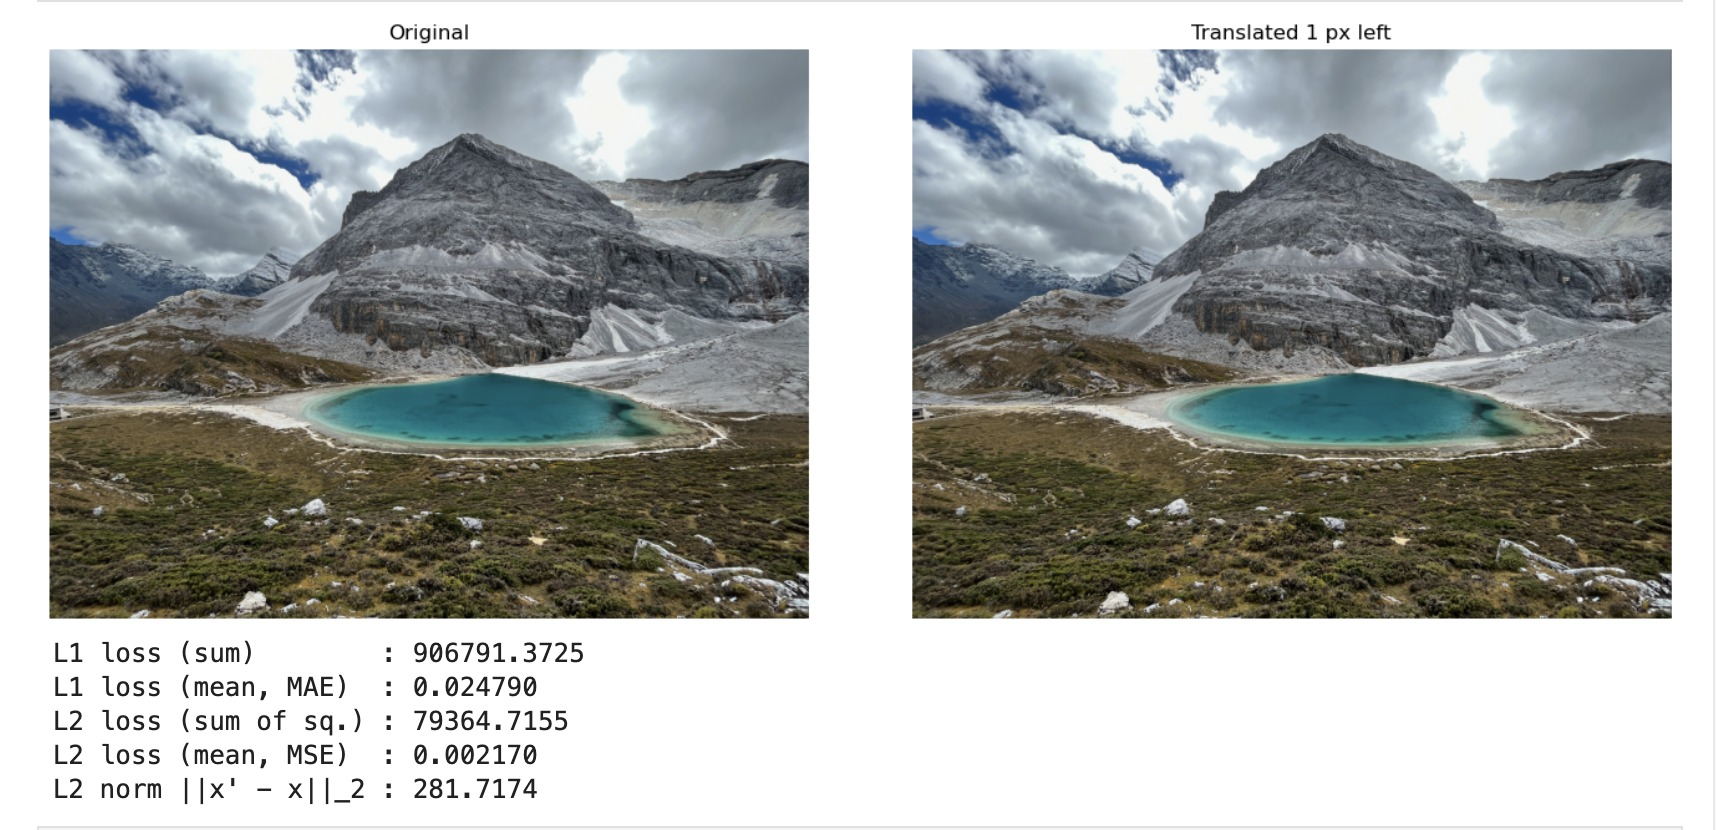
\includegraphics[width=\linewidth]{figs/p1_shift_pair.jpg}
\caption{Problem 1.1: the $4032{\times}3024$ test image (Daocheng Yading) and its 1-pixel left translation, with the $\ell_1$ and $\ell_2$ losses printed below. The two images are visually indistinguishable.}
\label{fig:photo}
\end{figure}

\begin{lstlisting}[float=tbp,caption={Shift and pixel losses (excerpt).},label={lst:shift}]
img = np.asarray(image_pil, np.float64) / 255.0  # [0,1]
shifted = np.zeros_like(img)
shifted[:, :-1] = img[:, 1:]      # pixel (r,c) <- (r,c+1)
diff = shifted - img
l1_sum, l1_mean = np.abs(diff).sum(), np.abs(diff).mean()
l2_sum, l2_mean = (diff**2).sum(), (diff**2).mean()
l2_norm = np.sqrt(l2_sum)          # ||x' - x||_2
\end{lstlisting}

\answer{$\ell_1 = 906{,}791$ (sum) or 0.0248 (mean); $\ell_2 = 79{,}365$ (sum of squares) or 0.00217 (MSE), with $\|x'-x\|_2=281.7$, for pixel values in $[0,1]$. The MSE equals that of adding Gaussian noise with $\sigma=\sqrt{0.00217}\approx0.047$, even though the shifted image looks identical to a human.}

\subsection{Change in VGG-16 feature space}
\label{sec:p1-2}
\paragraph{Feature taps.}
We use the ImageNet-pretrained VGG-16~\cite{simonyan2015vgg} from torchvision and read its features after the last ReLU of the first four blocks (\cref{fig:vgg}): \relu{1\_2}, \relu{2\_2}, \relu{3\_3} and \relu{4\_3}, which are \texttt{features[3]}, \texttt{[8]}, \texttt{[15]} and \texttt{[22]}. They span low-level edges (stride 1, 64 channels) to object-part detectors (stride 8, 512 channels), and they are the standard choices for perceptual losses~\cite{johnson2016perceptual,zhang2018lpips}. The image is ImageNet-normalized and processed at full resolution. To avoid an artificial edge at the zero-filled column, the original and the shifted image are compared on their common $3024{\times}4031$ region; this is why the pixel row of \cref{tab:shift} differs slightly from \cref{sec:p1-1}. For each tap $\phi$ we report $\ell_1$, MSE and the scale-free \emph{relative change} $\|\phi(x')-\phi(x)\|_2/\|\phi(x)\|_2$. Only the relative change can be compared across layers whose activations have very different magnitudes.

\begin{figure*}[t]
\centering
\begin{tikzpicture}[font=\scriptsize, node distance=2.2mm and 2.2mm, >={Stealth[length=1.5mm]},
  blk/.style={draw=black!60, rounded corners=1.5pt, fill=#1, minimum height=11mm, align=center, inner sep=2pt, text width=13.5mm},
  pool/.style={draw=black!50, fill=black!8, minimum height=11mm, minimum width=3.2mm, inner sep=0pt},
  tap/.style={draw=#1, line width=0.9pt, rounded corners=1.5pt, fill=#1!10, align=center, inner sep=2pt, text width=21mm}]
  \node[blk=white, text width=11mm] (in) {input\\$3{\times}H{\times}W$};
  \node[blk=black!3, right=of in] (b1) {conv1\_1, 1\_2\\64 ch};
  \node[pool, right=of b1] (p1) {};
  \node[blk=black!3, right=of p1] (b2) {conv2\_1, 2\_2\\128 ch};
  \node[pool, right=of b2] (p2) {};
  \node[blk=black!3, right=of p2] (b3) {conv3\_1--3\_3\\256 ch};
  \node[pool, right=of b3] (p3) {};
  \node[blk=black!3, right=of p3] (b4) {conv4\_1--4\_3\\512 ch};
  \node[pool, right=of b4] (p4) {};
  \node[blk=black!3, right=of p4] (b5) {conv5\_1--5\_3\\512 ch};
  \node[pool, right=of b5] (p5) {};
  \node[blk=black!3, right=of p5, text width=15mm] (fc) {FC 4096, 4096\\FC 1000\\(not used)};
  \foreach \a/\b in {in/b1,b1/p1,p1/b2,b2/p2,p2/b3,b3/p3,p3/b4,b4/p4,p4/b5,b5/p5,p5/fc} \draw[->] (\a) -- (\b);
  \foreach \p in {p1,p2,p3,p4,p5} \node[font=\tiny, below=0.5mm of \p] {pool};
  \node[tap=tapA, below=7mm of b1] (t1) {\textbf{\relu{1\_2}} \texttt{[3]}\\stride 1\\$64{\times}3024{\times}4031$};
  \node[tap=tapB, below=7mm of b2] (t2) {\textbf{\relu{2\_2}} \texttt{[8]}\\stride 2\\$128{\times}1512{\times}2015$};
  \node[tap=tapC, below=7mm of b3] (t3) {\textbf{\relu{3\_3}} \texttt{[15]}\\stride 4\\$256{\times}756{\times}1007$};
  \node[tap=tapD, below=7mm of b4] (t4) {\textbf{\relu{4\_3}} \texttt{[22]}\\stride 8\\$512{\times}378{\times}503$};
  \foreach \b/\t/\c in {b1/t1/tapA,b2/t2/tapB,b3/t3/tapC,b4/t4/tapD} {
    \fill[\c] (\b.south) circle (1.1pt);
    \draw[->, \c, line width=0.8pt] (\b.south) -- (\t.north);}
  \node[anchor=west, align=left, text width=36mm, font=\scriptsize] at ($(t4.east)+(4mm,0)$)
    {Four feature taps (colored) read after the last ReLU of blocks 1--4. \texttt{[k]} = index in \texttt{torchvision} \texttt{vgg16().features}; shapes are for the shifted $3024{\times}4031$ photo.};
\end{tikzpicture}
\caption{VGG-16 with the four feature-extraction points used in Problems 1.2 and 1.3. Each block is a stack of $3{\times}3$ conv + ReLU layers; each max-pool halves the resolution, so the stride doubles from one tap to the next.}
\label{fig:vgg}
\end{figure*}

\begin{table}[t]
\centering\footnotesize\setlength{\tabcolsep}{4pt}
\begin{tabular}{@{}lrrrr@{}}
\toprule
Space & Shape & mean $\ell_1$ & MSE & rel.\ change \\
\midrule
pixels & $3{\times}3024{\times}4031$ & 0.0247 & 0.00212 & \textbf{0.090} \\
\textcolor{tapA}{\relu{1\_2}} & $64{\times}3024{\times}4031$ & 0.254 & 0.447 & 0.590 \\
\textcolor{tapB}{\relu{2\_2}} & $128{\times}1512{\times}2015$ & 0.378 & 1.120 & 0.557 \\
\textcolor{tapC}{\relu{3\_3}} & $256{\times}756{\times}1007$ & 0.229 & 0.663 & 0.379 \\
\textcolor{tapD}{\relu{4\_3}} & $512{\times}378{\times}503$ & 0.045 & 0.049 & 0.317 \\
\bottomrule
\end{tabular}
\caption{Change caused by a 1-pixel left shift, in pixel space and at the four VGG-16 taps. $\ell_1$ and MSE are not comparable across rows (activation scales differ), so we compare the relative change.}
\label{tab:shift}
\end{table}

\begin{figure*}[t]
\centering
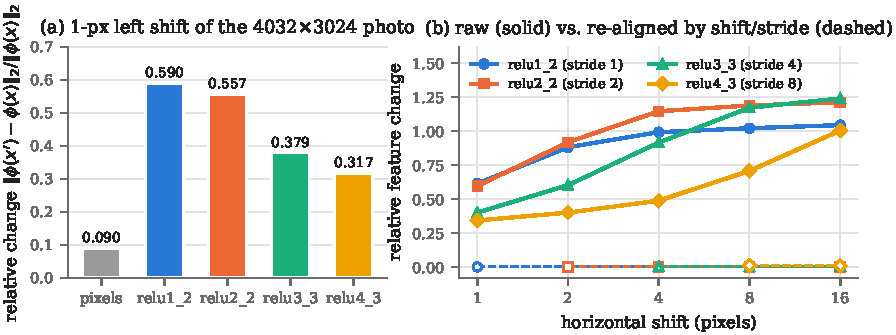
\includegraphics[width=\linewidth]{figs/p1_shift.pdf}
\caption{(a) Relative change for a 1-pixel shift: the features change 3.5--6.6$\times$ more than the pixels. (b) Verification experiment: relative change \vs shift size (solid). When the shifted feature map is re-aligned by $\text{shift}/\text{stride}$ cells, which is only possible when the shift is a multiple of the layer's stride, the change drops to $\le 0.009$ (dashed). The features are therefore exactly shift-\emph{equivariant} on their own sampling grid, and the 1-pixel change is caused by sampling (aliasing).}
\label{fig:shift}
\end{figure*}

\paragraph{Observations.}
\cref{tab:shift} and \cref{fig:shift}a show that the shift barely changes the pixels (9.0\%) but changes every feature map substantially. The change is largest at \relu{1\_2} (59\%) and \emph{decreases} with depth to 32\% at \relu{4\_3}. In relative terms, the features are 3.5--6.6$\times$ \emph{more} sensitive to the translation than the pixel losses. This contradicts the common intuition that ``deep features are shift-invariant.'' We ran four checks to explain it:
\begin{enumerate}[nosep,leftmargin=*]
\item \textbf{Identical inputs} give exactly zero change at all taps, so the pipeline is correct.
\item \textbf{Aliasing.} Shifting a feature map back by $\text{shift}/\text{stride}$ cells, possible only when the shift is a multiple of the stride, makes the change vanish ($\le 0.009$, \cref{fig:shift}b). The features are equivariant on their own grid. A 1-pixel shift is not a multiple of the stride after pooling, so max-pooling and subsampling sample different pixels and produce a different map~\cite{zhang2019blurpool}. Even \relu{1\_2} (stride 1) changes by 0.61, because its edge maps are compared at the same coordinates, where sharp edges no longer overlap.
\item \textbf{Edges dominate.} Pixel relative change is 0.145 for raw pixels\footnote{This check ran on a resized copy, hence 0.145 instead of the 0.090 of \cref{tab:shift}.}, 0.309 after removing the mean, and 0.611 for a high-pass (edge-only) image. The edge-only value matches \relu{1\_2} (0.613): early VGG layers behave like edge detectors, and the pixel loss looks small only because the smooth (DC) content dominates the pixel norm.
\item \textbf{Sparsity and pooling.} The fraction of exactly-zero activations grows from 55\% (\relu{1\_2}) to 70\%, 85\% and 92\% (\relu{4\_3}). When a few sparse peaks move by one cell, both the old and the new location change. Averaging each channel over space (global average pooling) removes this: the channel means change by only 0.05\%, 2.2\%, 2.5\% and 3.8\%.
\end{enumerate}

\paragraph{Choice of perceptual feature.}
For a perceptual loss we would use a channel-normalized, multi-layer distance on \relu{2\_2} and \relu{3\_3} (an LPIPS-style sum~\cite{zhang2018lpips}), computed after a small anti-aliasing blur. \relu{2\_2} is the layer Johnson~\etal use for feature reconstruction~\cite{johnson2016perceptual}. It keeps half-resolution detail, which tasks such as super-resolution need. \relu{3\_3} adds mid-level texture and part information and is 32\% less shift-sensitive than \relu{1\_2}. \relu{4\_3} is the least shift-sensitive tap, but at 1/8 resolution and 92\% sparsity it is too coarse to judge fine detail. Our measurements also show that spatial pooling makes VGG statistics almost shift-invariant ($\le$3.8\%), so the blur or pooling step is what makes the loss tolerant to imperceptible misalignment.

\answer{Pixel losses report a small change (9\% relative), while raw VGG features report a large one (32--59\%) that decreases with depth. The cause is aliasing from stride and max-pooling, not semantics: on an aligned grid the change is $\le$0.9\%, and pooled channel statistics change $\le$3.8\%. We recommend \relu{2\_2}+\relu{3\_3}, channel-normalized and slightly blurred or pooled before comparison.}

\subsection{Robustness to additive noise}
\label{sec:p1-3}
We add i.i.d.\ Gaussian noise with $\sigma\in\{0.01,0.02,0.05,0.1,0.2,0.3\}$ to the $[0,1]$ image (PSNR from 40 to 12\,dB) and measure the relative change in pixel space and at all four taps. \cref{fig:noise-maps} shows the qualitative result as per-location change maps. \cref{fig:noise} and \cref{tab:noise} show the quantitative result.

\begin{figure}[t]
\centering
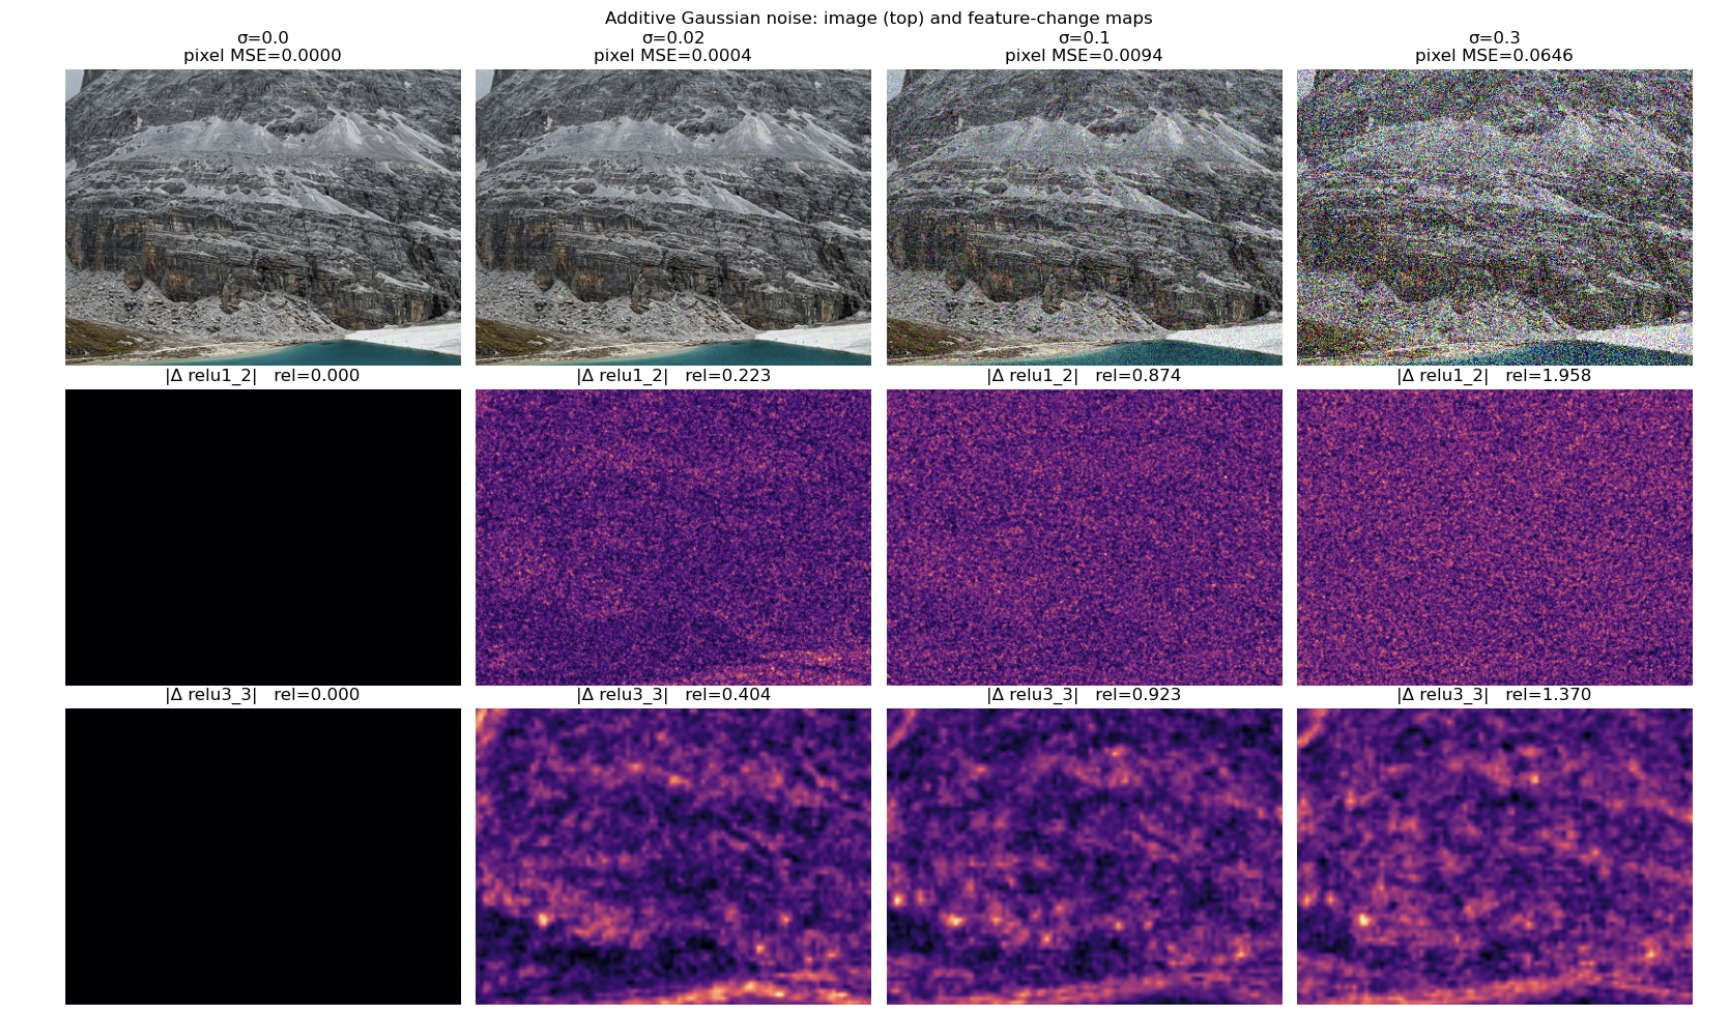
\includegraphics[width=\linewidth]{figs/p1_noise_maps.jpg}
\caption{Qualitative noise test. Top: noisy images ($\sigma=0, 0.02, 0.1, 0.3$). Middle and bottom: per-location feature-change maps $|\Delta|$ for \relu{1\_2} and \relu{3\_3}. The \relu{1\_2} change is spatially uniform (it reacts to every noisy pixel). The \relu{3\_3} change concentrates on textured regions such as the rock strata and the lake shore.}
\label{fig:noise-maps}
\end{figure}

\begin{figure}[t]
\centering
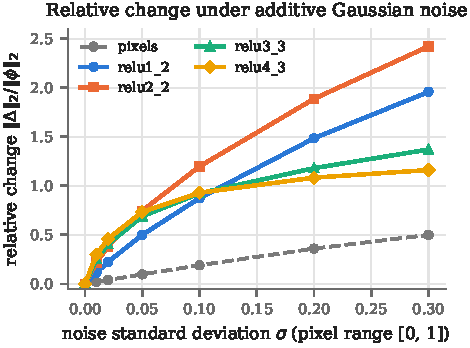
\includegraphics[width=\linewidth]{figs/p1_noise.pdf}
\caption{Quantitative noise test: relative change \vs noise level in pixel space and at the four VGG-16 taps. Deeper taps saturate; shallow taps keep growing.}
\label{fig:noise}
\end{figure}

\begin{table}[t]
\centering\footnotesize\setlength{\tabcolsep}{3.2pt}
\begin{tabular}{@{}lcccccc@{}}
\toprule
$\sigma$ & 0.01 & 0.02 & 0.05 & 0.1 & 0.2 & 0.3 \\
PSNR (dB) & 40.0 & 34.0 & 26.1 & 20.3 & 14.7 & 11.9 \\
pixel MSE & 0.0001 & 0.0004 & 0.0024 & 0.0094 & 0.0336 & 0.0646 \\
\midrule
pixels & 0.020 & 0.039 & 0.097 & 0.190 & 0.360 & 0.499 \\
\textcolor{tapA}{\relu{1\_2}} & 0.114 & 0.223 & 0.499 & 0.874 & 1.485 & 1.958 \\
\textcolor{tapB}{\relu{2\_2}} & 0.217 & 0.378 & 0.746 & 1.197 & 1.887 & \textbf{2.421} \\
\textcolor{tapC}{\relu{3\_3}} & 0.251 & 0.404 & 0.688 & 0.924 & 1.180 & 1.370 \\
\textcolor{tapD}{\relu{4\_3}} & \textbf{0.296} & 0.458 & 0.733 & 0.929 & 1.083 & \textbf{1.161} \\
\bottomrule
\end{tabular}
\caption{Relative change $\|\Delta\|_2/\|\phi\|_2$ under additive Gaussian noise. From $\sigma{=}0.01$ to $0.3$ it grows 25$\times$ for pixels, 17$\times$ for \relu{1\_2}, 11$\times$ for \relu{2\_2}, 5.5$\times$ for \relu{3\_3} and 3.9$\times$ for \relu{4\_3}.}
\label{tab:noise}
\end{table}

\paragraph{Observations.}
(i)~Every feature space is far more sensitive than pixel space: at $\sigma{=}0.02$ (PSNR 34\,dB, barely visible) the pixels change by 3.9\% but the features by 22--46\%. For \relu{3\_3}, this weak noise is as large a change as the 1-pixel shift (0.40 \vs 0.38), while for pixels the noise is less than half the shift (0.039 \vs 0.090).
(ii)~For weak noise, sensitivity \emph{increases} with depth ($\sigma{=}0.01$: 0.11, 0.22, 0.25, 0.30 from \relu{1\_2} to \relu{4\_3}): faint noise excites the texture detectors.
(iii)~Deeper layers \emph{saturate}. Over a 30$\times$ increase in $\sigma$, the change grows 17$\times$ at \relu{1\_2} but only 3.9$\times$ at \relu{4\_3}. Above $\sigma{\approx}0.1$ the order reverses: at $\sigma{=}0.3$, \relu{4\_3} (1.16) and \relu{3\_3} (1.37) are the most robust and \relu{2\_2} (2.42) the least.
(iv)~Qualitatively, the \relu{3\_3} change follows image structure, while the \relu{1\_2} change looks like the noise itself.

\answer{No feature is noise-invariant, and all of them react more than pixels. Shallow taps behave like a pixel loss and keep growing with $\sigma$. Deep taps (\relu{3\_3}, \relu{4\_3}) are the most robust to moderate and strong noise (relative change 1.16--1.37 at $\sigma{=}0.3$, \vs 1.96--2.42 for shallow taps) and localize the damage to textured regions, but they are the most sensitive to faint noise. For noisy inputs, our perceptual loss of \cref{sec:p1-2} should therefore weight \relu{3\_3} more than \relu{2\_2}.}

\subsection{A perceptual feature robust to atmospheric turbulence}
\label{sec:p1-4}
\paragraph{Why standard features fail.}
DAATSim~\cite{saha2025daatsim} models turbulence as a smooth random \emph{tilt} (each region shifts by a different sub-pixel to few-pixel amount) plus spatially varying \emph{blur}. \cref{sec:p1-2} showed that VGG features are dominated by aliasing under exactly such small, non-stride-aligned shifts. We therefore expect standard perceptual features to treat turbulence as a large change, and we design against that failure mode.

\paragraph{Dataset.}
We took the 100 diverse high-resolution photos of the DIV2K validation set~\cite{agustsson2017div2k}, cut 8 random $256{\times}256$ crops from each (800 clean images), and split them \emph{by source photo} into 640 training and 160 test images. Each training crop has 3 turbulent versions, with $r_0$ drawn uniformly from $[0.02,0.1]$, \ie $D/r_0\in[2,10]$ (smaller $r_0$ = stronger turbulence). Each test crop has one version at each of $D/r_0\in\{2,4,6.7,10,20\}$. The strongest level, $D/r_0{=}20$, lies outside the training range and tests generalization (\cref{fig:turb-data}). We wrapped DAATSim's tilt and blur stages (uniform depth) so that it renders one turbulent frame per image.

\begin{figure}[t]
\centering
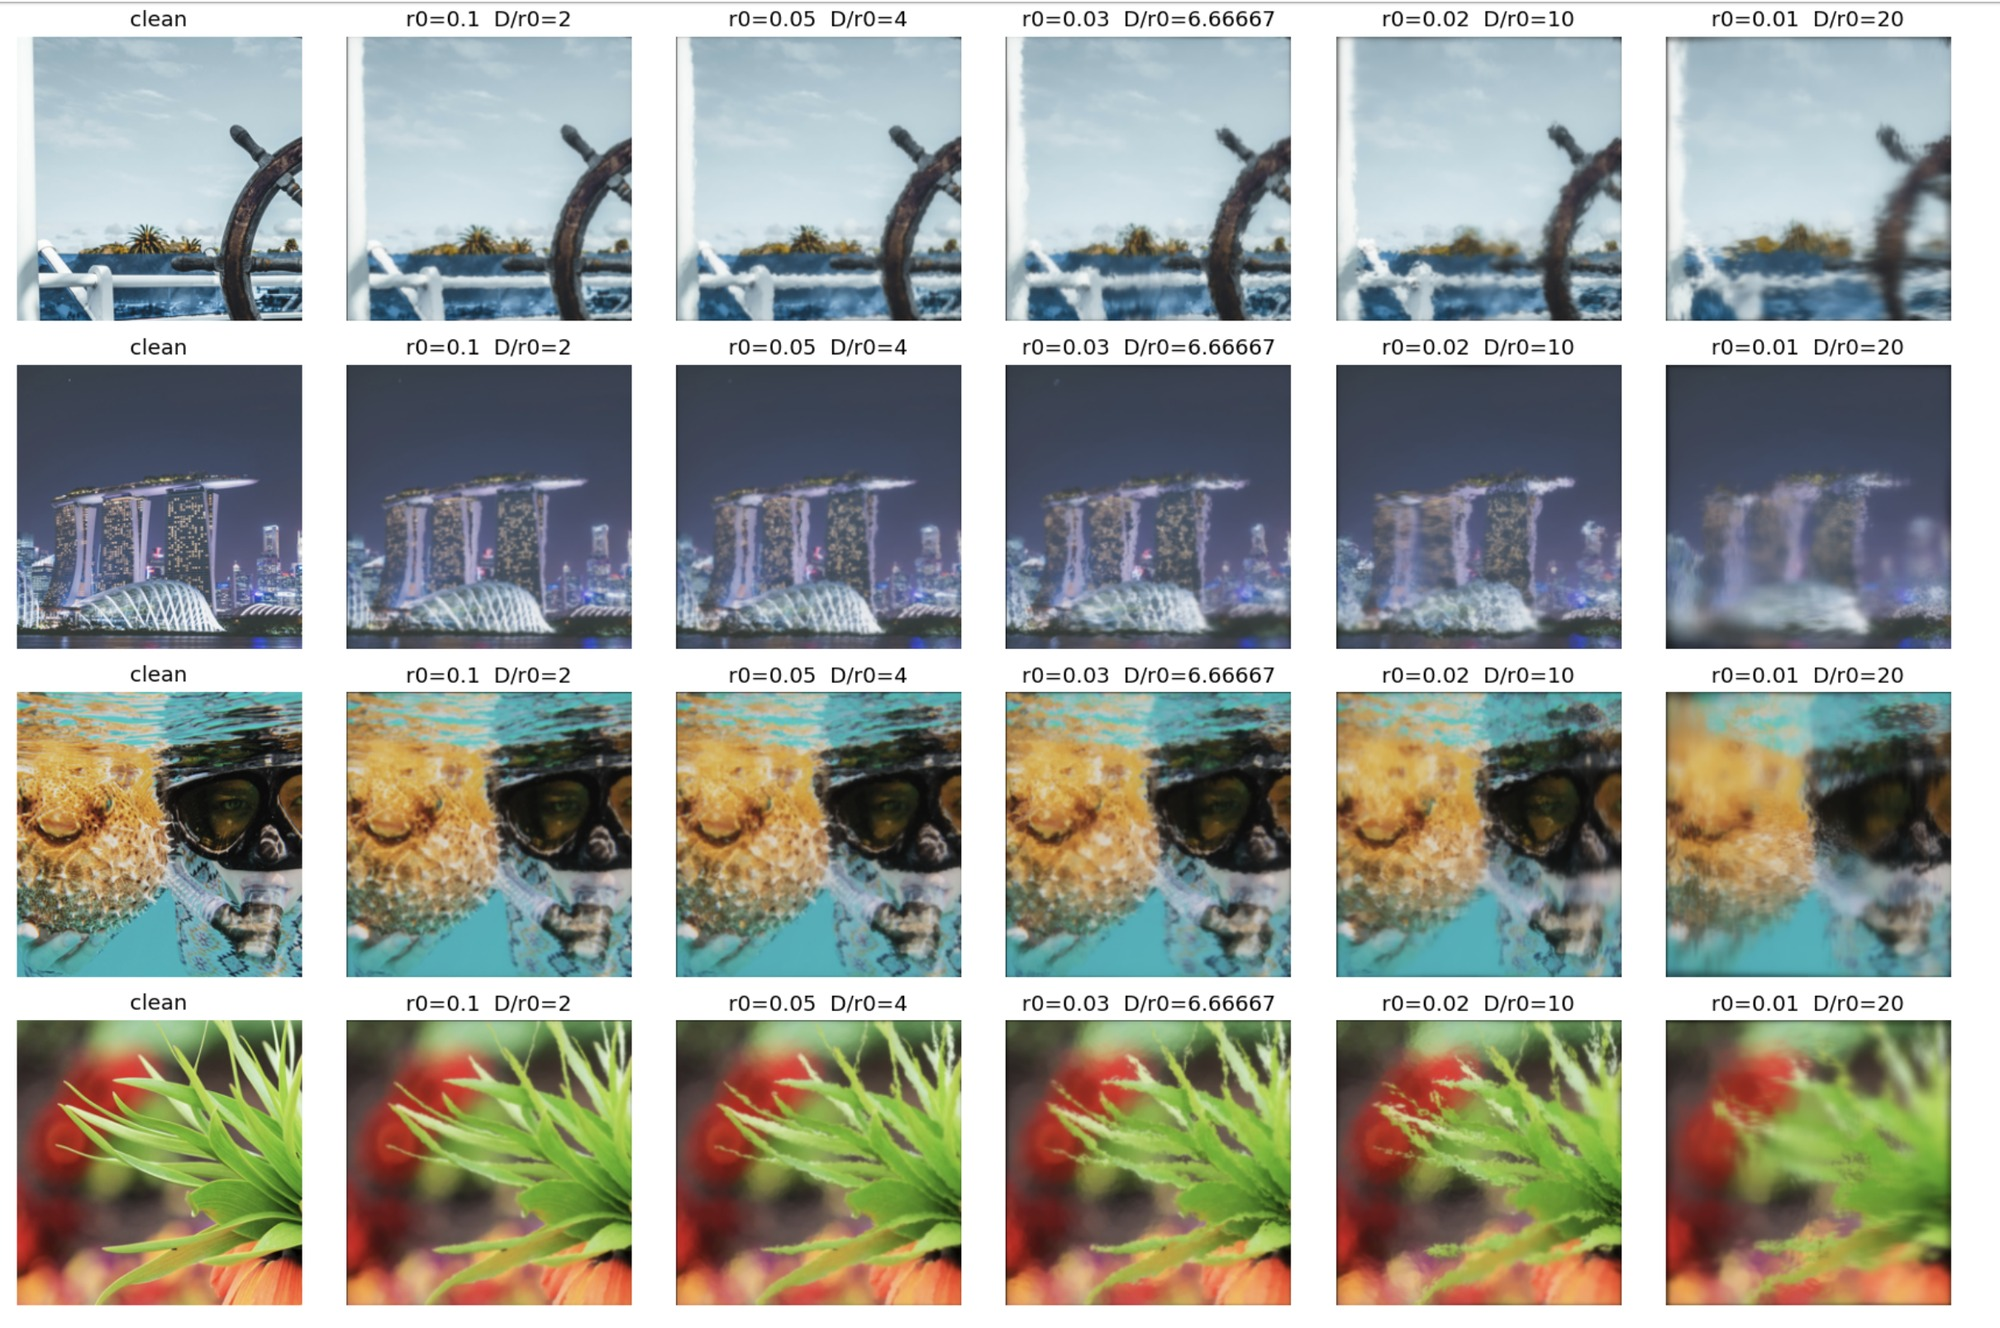
\includegraphics[width=\linewidth]{figs/p1_turb_dataset.jpg}
\caption{Examples from our turbulence dataset: clean DIV2K crops (left) and their DAATSim versions at the five test strengths ($D/r_0$ from 2 to 20). Tilt bends straight edges; blur grows with $D/r_0$.}
\label{fig:turb-data}
\end{figure}

\paragraph{Proposed feature.}
Our feature $z=g(\phi_{\text{AA}}(x))$ has three parts:
\begin{enumerate}[nosep,leftmargin=*]
\item \textbf{Anti-aliased trunk.} A frozen ImageNet VGG-16 in which every max-pool is replaced by max$\rightarrow$blur$\rightarrow$subsample (BlurPool~\cite{zhang2019blurpool}). This directly targets the aliasing measured in \cref{sec:p1-2}.
\item \textbf{Multi-scale head $g$.} \relu{2\_2} (BlurPool-downsampled) and \relu{3\_3} are concatenated and passed through two $3{\times}3$ conv layers, giving a 128-dimensional, unit-normalized feature map at 1/4 resolution (1.18M trainable parameters). The $3{\times}3$ receptive field lets the head learn to tolerate local tilt.
\item \textbf{Dense contrastive training.} For a clean image $x$ and its turbulent version $T(x)$ we sample 64 locations per image and minimize the symmetric InfoNCE loss~\cite{oord2018cpc,wang2021densecl}:
\begin{equation}
\mathcal{L} = -\frac{1}{|P|}\sum_{p\in P}\log\frac{\exp(z_p^{\top}z'_p/\tau)}{\sum_{q\in P}\exp(z_p^{\top}z'_q/\tau)} ,
\end{equation}
where $z=g(x)$, $z'=g(T(x))$, $\tau=0.1$, and $P$ contains the sampled locations of all images in the batch. The positive pair (same location) teaches invariance to turbulence. The negatives (other locations and other images) prevent the trivial constant solution and keep the feature sensitive to real content changes.
\end{enumerate}
Training uses AdamW (lr $10^{-3}$, cosine schedule), batch 16 and 30 epochs. We compare against two ablations: \emph{no anti-aliasing} (original max-pooling) and \emph{invariance-only} (pull positives together without negatives).

\begin{lstlisting}[float=tbp,caption={Dense InfoNCE loss on sampled feature locations.},label={lst:infonce}]
def dense_infonce(za, zb, n_loc=64, tau=0.1):
    # za, zb: B×D×h×w unit-norm maps of x and T(x)
    idx = sample_locations(za, n_loc)  # same p in both
    qa = gather(za, idx).reshape(-1, D)   # (B*n_loc)×D
    qb = gather(zb, idx).reshape(-1, D)
    logits = qa @ qb.t() / tau     # positives on diagonal
    t = torch.arange(len(qa), device=za.device)
    ce = F.cross_entropy
    return 0.5 * (ce(logits, t) + ce(logits.t(), t))
\end{lstlisting}

\paragraph{Evaluation protocol.}
A feature that ignores everything is perfectly ``invariant'' and useless, so invariance alone is not a valid metric. For each test image $x$ we compare $d(x,T(x))$, which should be small, with $d(x,\text{edit}(x))$, where a $64{\times}64$ patch is replaced by content from another scene, which should be large. Our main metric is
$\text{AUC}_{\text{edit}}=P\big(d(x,T(x))<d(x,\text{edit}(x))\big)$: 1.0 means turbulence is always judged a smaller change than a real edit, and 0.5 is chance. We also report the \emph{distance ratio}, the median $d(x,T(x))$ divided by the median distance between two \emph{different} images (lower = more invariant). Baselines are pixel MSE, blurred pixels (Gaussian, $\sigma{=}2$), the four VGG taps of \cref{sec:p1-2}, an LPIPS-style 4-tap sum~\cite{zhang2018lpips}, and an untrained anti-aliased VGG.

\begin{figure*}[t]
\centering
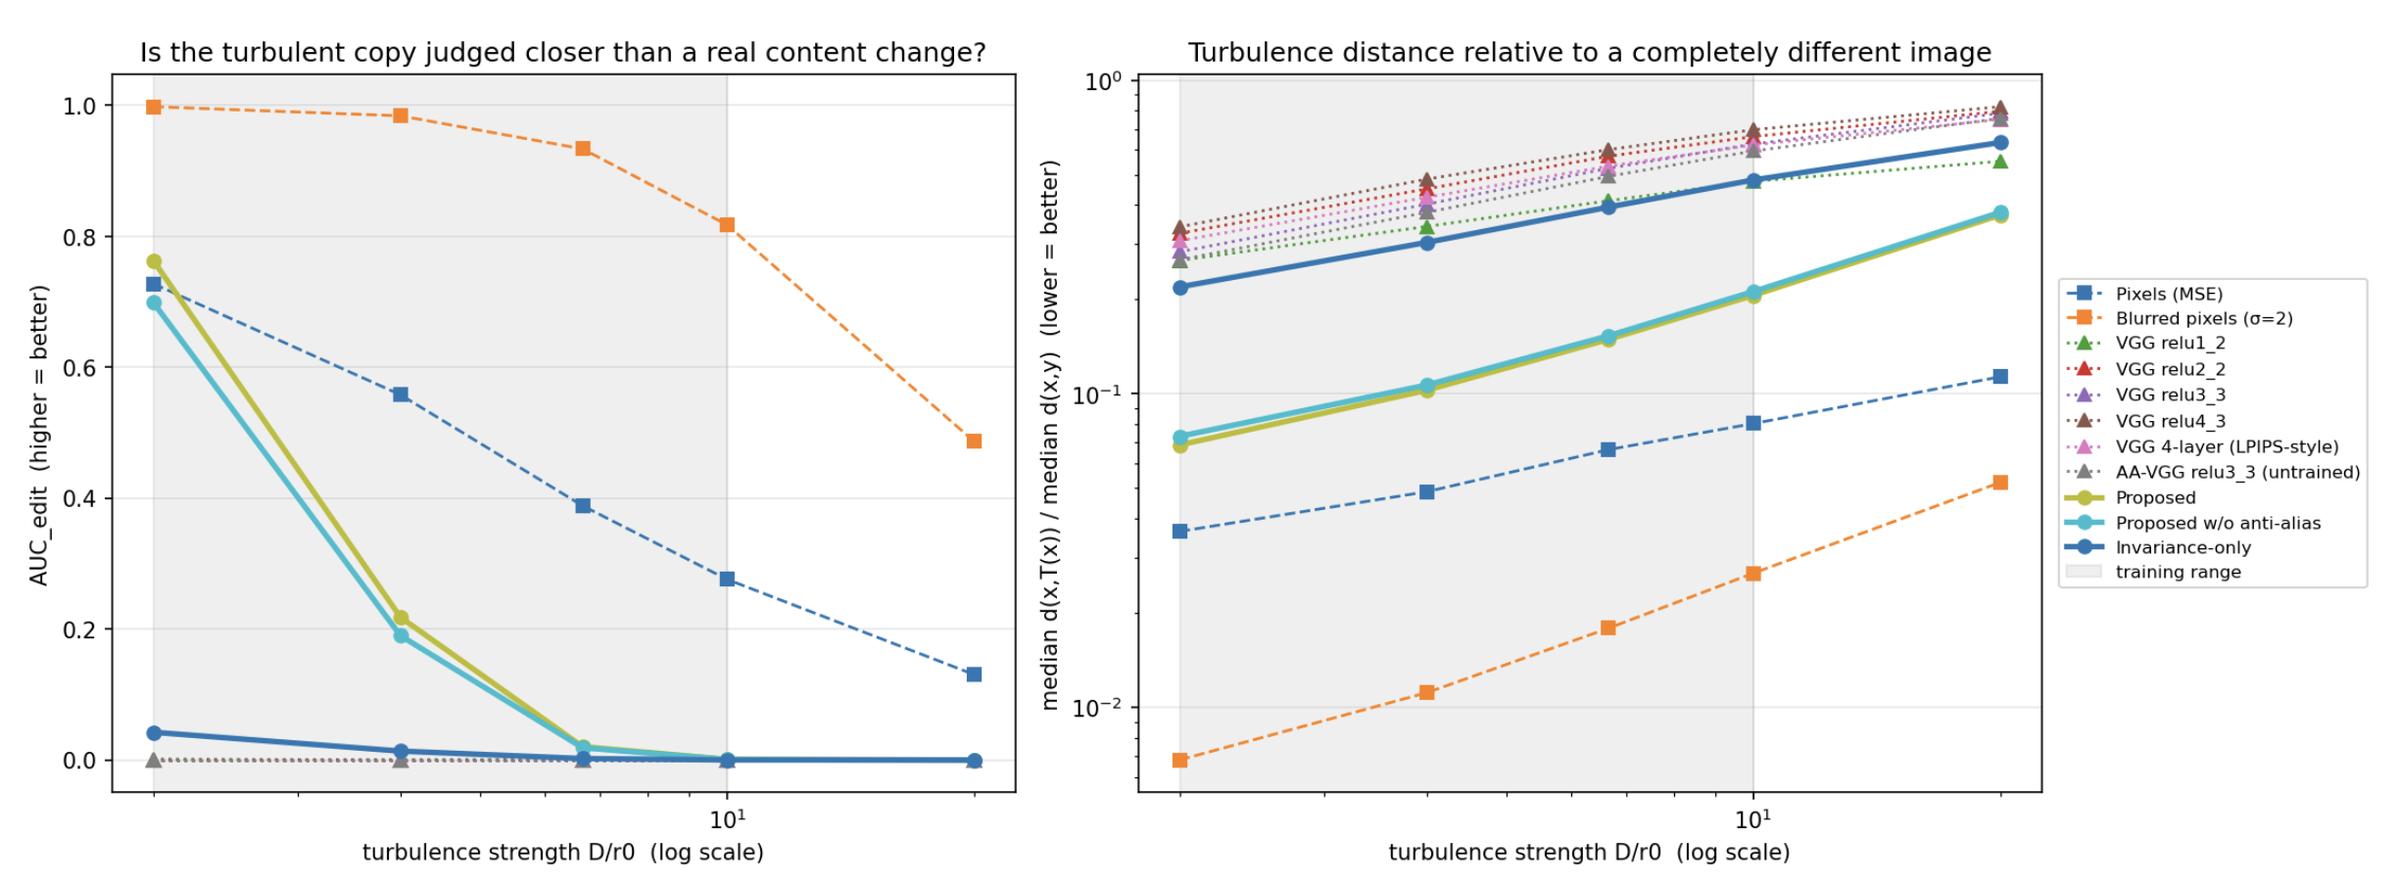
\includegraphics[width=0.93\linewidth]{figs/p1_turb_quant.png}
\caption{Turbulence robustness on the 160 held-out test images \vs turbulence strength (gray band = training range). Left: AUC$_\text{edit}$, the probability that the turbulent copy is judged closer than a $64{\times}64$ content edit (higher = better). Right: median turbulence distance divided by the median distance to a different image (log scale, lower = more invariant).}
\label{fig:turb}
\end{figure*}

\begin{figure*}[t]
\centering
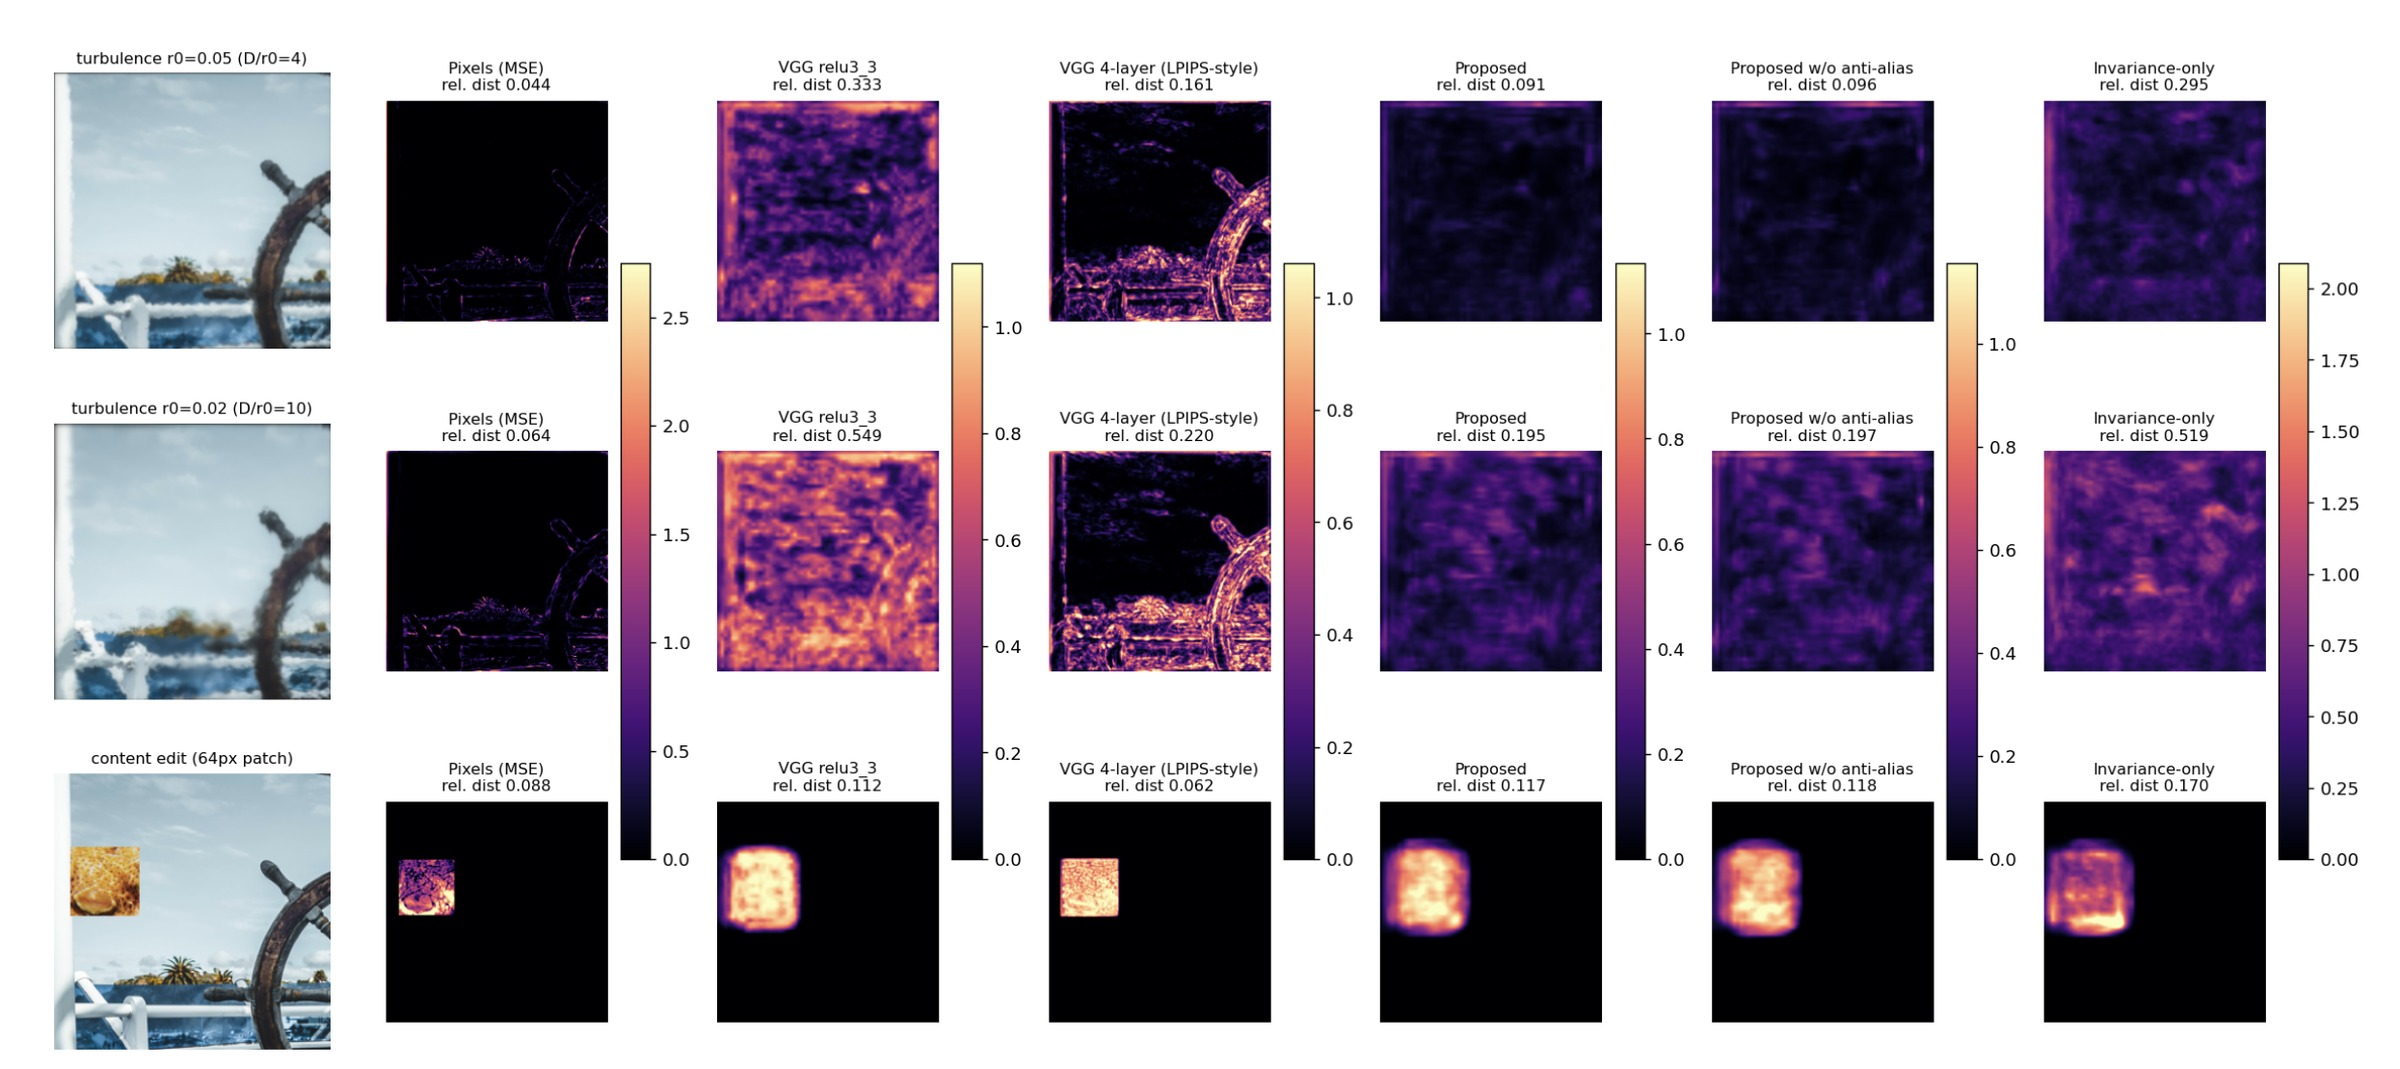
\includegraphics[width=\linewidth]{figs/p1_turb_qual.jpg}
\caption{Where each feature changes, for turbulence at $D/r_0{=}4$ (top) and $D/r_0{=}10$ (middle) and for a $64{\times}64$ content edit (bottom). Values are divided by each feature's distance to a different image and share one color scale per column; ``rel.\ dist'' is the image-level distance. Ideal: dark under turbulence, bright only on the edited patch.}
\label{fig:turb-qual}
\end{figure*}

\begin{table}[t]
\centering\footnotesize\setlength{\tabcolsep}{3pt}
\resizebox{\linewidth}{!}{%
\begin{tabular}{@{}lccccc|cc@{}}
\toprule
 & \multicolumn{5}{c|}{AUC$_\text{edit}$ ($\uparrow$) at $D/r_0=$} & \multicolumn{2}{c}{ratio ($\downarrow$)} \\
Feature & 2 & 4 & 6.7 & 10 & 20$^\dagger$ & 2 & 20$^\dagger$ \\
\midrule
pixels (MSE) & 0.728 & 0.558 & 0.388 & 0.276 & 0.130 & 0.036 & 0.113 \\
blurred pixels & \textbf{0.998} & \textbf{0.984} & \textbf{0.934} & \textbf{0.817} & \textbf{0.486} & \textbf{0.007} & \textbf{0.052} \\
VGG taps / LPIPS / AA-VGG & $\le$0.001 & 0.000 & 0.000 & 0.000 & 0.000 & 0.27--0.34 & 0.55--0.82 \\
\midrule
Proposed & 0.763 & 0.218 & 0.020 & 0.001 & 0.000 & 0.069 & 0.372 \\
\quad w/o anti-aliasing & 0.699 & 0.190 & 0.019 & 0.001 & 0.000 & 0.073 & 0.380 \\
\quad invariance-only & 0.042 & 0.014 & 0.002 & 0.000 & 0.000 & 0.219 & 0.634 \\
\bottomrule
\end{tabular}}
\caption{Turbulence results on the 160 test images (from \texttt{metrics.csv}). Every feature judges the turbulent copy closer than a \emph{different} image ($\text{AUC}\ge0.998$, not shown). $^\dagger$Stronger than any training turbulence. ``VGG taps / LPIPS / AA-VGG'' covers the four single VGG taps, the LPIPS-style sum and the untrained anti-aliased VGG, which all behave alike.}
\label{tab:turb}
\end{table}

\paragraph{Results.}
\cref{fig:turb,fig:turb-qual} and \cref{tab:turb} show four findings.
(i)~\textbf{Standard perceptual features fail completely.} All VGG taps, the LPIPS-style sum and the untrained anti-aliased VGG have AUC$_\text{edit}\approx0$ at every strength: they always judge even weak turbulence a \emph{larger} change than replacing a whole $64{\times}64$ patch. In \cref{fig:turb-qual}, \relu{3\_3} lights up across the whole image under turbulence (rel.\ dist 0.33 at $D/r_0{=}4$ \vs 0.11 for the edit).
(ii)~\textbf{The proposed feature is much more robust than VGG.} It reaches AUC$_\text{edit}=0.76$ at $D/r_0{=}2$ and lowers the distance ratio 4--5$\times$ (0.07 \vs 0.27--0.34). Its change maps are dark under turbulence and bright on the edited patch; at $D/r_0{=}4$ it ranks the turbulent copy closer than the edit (0.091 \vs 0.117), which none of the VGG features does. Anti-aliasing helps slightly but consistently (0.76 \vs 0.70), and the contrastive negatives are essential: without them the feature cannot separate edits from turbulence (AUC$\le$0.04).
(iii)~\textbf{But it degrades quickly.} AUC$_\text{edit}$ falls to 0.22 at $D/r_0{=}4$ and to $\approx$0 from $D/r_0{=}6.7$, even inside the training range, and it does not generalize to $D/r_0{=}20$.
(iv)~\textbf{A blurred-pixel distance is the best feature here} (AUC 1.00 to 0.82 inside the training range, 0.49 at $D/r_0{=}20$).

\paragraph{Why the problem is hard.}
The edit changes $64^2/256^2=1/16$ of the image, whereas turbulence changes \emph{every} location. For an image-level distance to rank turbulence below the edit, the per-location response to turbulence must be more than about 16$\times$ smaller than the response to replaced content. VGG features respond strongly to edges and texture, which is exactly what tilt displaces and blur removes (\cref{sec:p1-2}, check~3), so they fail by a wide margin. Our learned head shrinks the turbulence response enough for weak tilt, but its $3{\times}3$ receptive field at 1/4 resolution cannot absorb the larger displacements of stronger turbulence. Low-pass filtering wins because it discards precisely the high frequencies that turbulence corrupts, while the edit changes low-frequency color and brightness. Two directions follow from this: computing the learned feature on a low-pass pyramid, and matching features within a local search window (min-distance over small displacements) instead of at fixed coordinates. Two limitations remain: a turbulence-invariant feature is also less sensitive to blur in general, which a restoration loss \emph{should} penalize, and both training and testing use DAATSim in uniform-depth mode, so the sim-to-real gap is untested.

\answer{We built a turbulence-robust feature from an anti-aliased VGG trunk, a multi-scale head and a dense contrastive loss. Under weak turbulence it is far more robust than every standard perceptual feature (AUC$_\text{edit}$ 0.76 \vs 0.00; 4--5$\times$ lower distance ratio). It does not hold up under strong turbulence, where a simple blurred-pixel distance is best. The experiments show that robustness requires suppressing the high-frequency content that VGG features are built on.}

%%%%%%%%%%%%%%%%%%%%%%%%%%%%%%%%%%%%%%%%%%%%%%%%%%%%%%%%%%%%%%%%%%%%%%%%%%%%%%%%%%%%%%%%%%%%%%%%%%%
\section{Problem 2: ViT on the PV image dataset}
\label{sec:p2}

\subsection{Data pre-processing and augmentation}
\label{sec:p2-1}
\paragraph{Dataset.}
We use the RaptorMaps InfraredSolarModules dataset~\cite{millendorf2020pv}: 20{,}000 single-channel infrared images of $24{\times}40$ pixels in 12 classes (11 anomaly types and No-Anomaly). Labels come from \texttt{module\_metadata.json}. The data is highly imbalanced: No-Anomaly has 10{,}000 images and Diode-Multi only 175 (\cref{fig:pv-counts}). \cref{fig:pv-samples} shows five samples with their labels.

\paragraph{Unsharp masking.}
Every image is sharpened with an unsharp mask~\cite{gonzalez2018dip}, $\tilde x = x + a\,(x - G_r * x)$, where $G_r$ is a Gaussian blur of radius $r{=}1$, the amount is $a{=}1.5$, and differences below 2 gray levels are skipped so that flat regions and noise are not amplified. The radius is 1 rather than the usual 2 because the images are tiny. As \cref{fig:unsharp} shows, hot spots become brighter with sharper boundaries, and shadow edges and the cell grid become more visible. Faint noise and compression artifacts are also boosted.

\paragraph{Balancing.}
Classes above 2{,}500 images (only No-Anomaly) are randomly down-sampled. For every other class all originals are kept, and new images are generated from random unsharpened originals by a random non-empty combination of horizontal flip, vertical flip and color jitter. Because the images are grayscale, the jitter changes only brightness and contrast ($\pm$20\%). Images are saved as PNG to avoid JPEG artifacts at this size. \cref{tab:pv} summarizes the result: 12{,}500 originals plus 17{,}500 augmented images = 30{,}000. Every augmented image records its source image (\texttt{source\_id}). The split is done by source image per class (70/15/15\%), so an original and all its copies always land in the same split, which avoids train/test leakage. The split has 21{,}011 / 4{,}526 / 4{,}463 images, of which 8{,}750 / 1{,}875 / 1{,}875 are originals.

\begin{figure}[t]
\centering
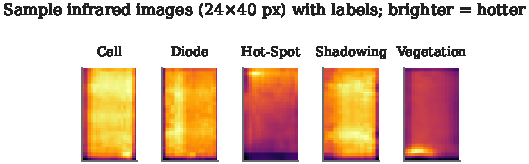
\includegraphics[width=\linewidth]{figs/p2_samples.pdf}
\caption{Five samples from the PV dataset with their labels (false color: brighter = hotter).}
\label{fig:pv-samples}
\end{figure}

\begin{figure}[t]
\centering
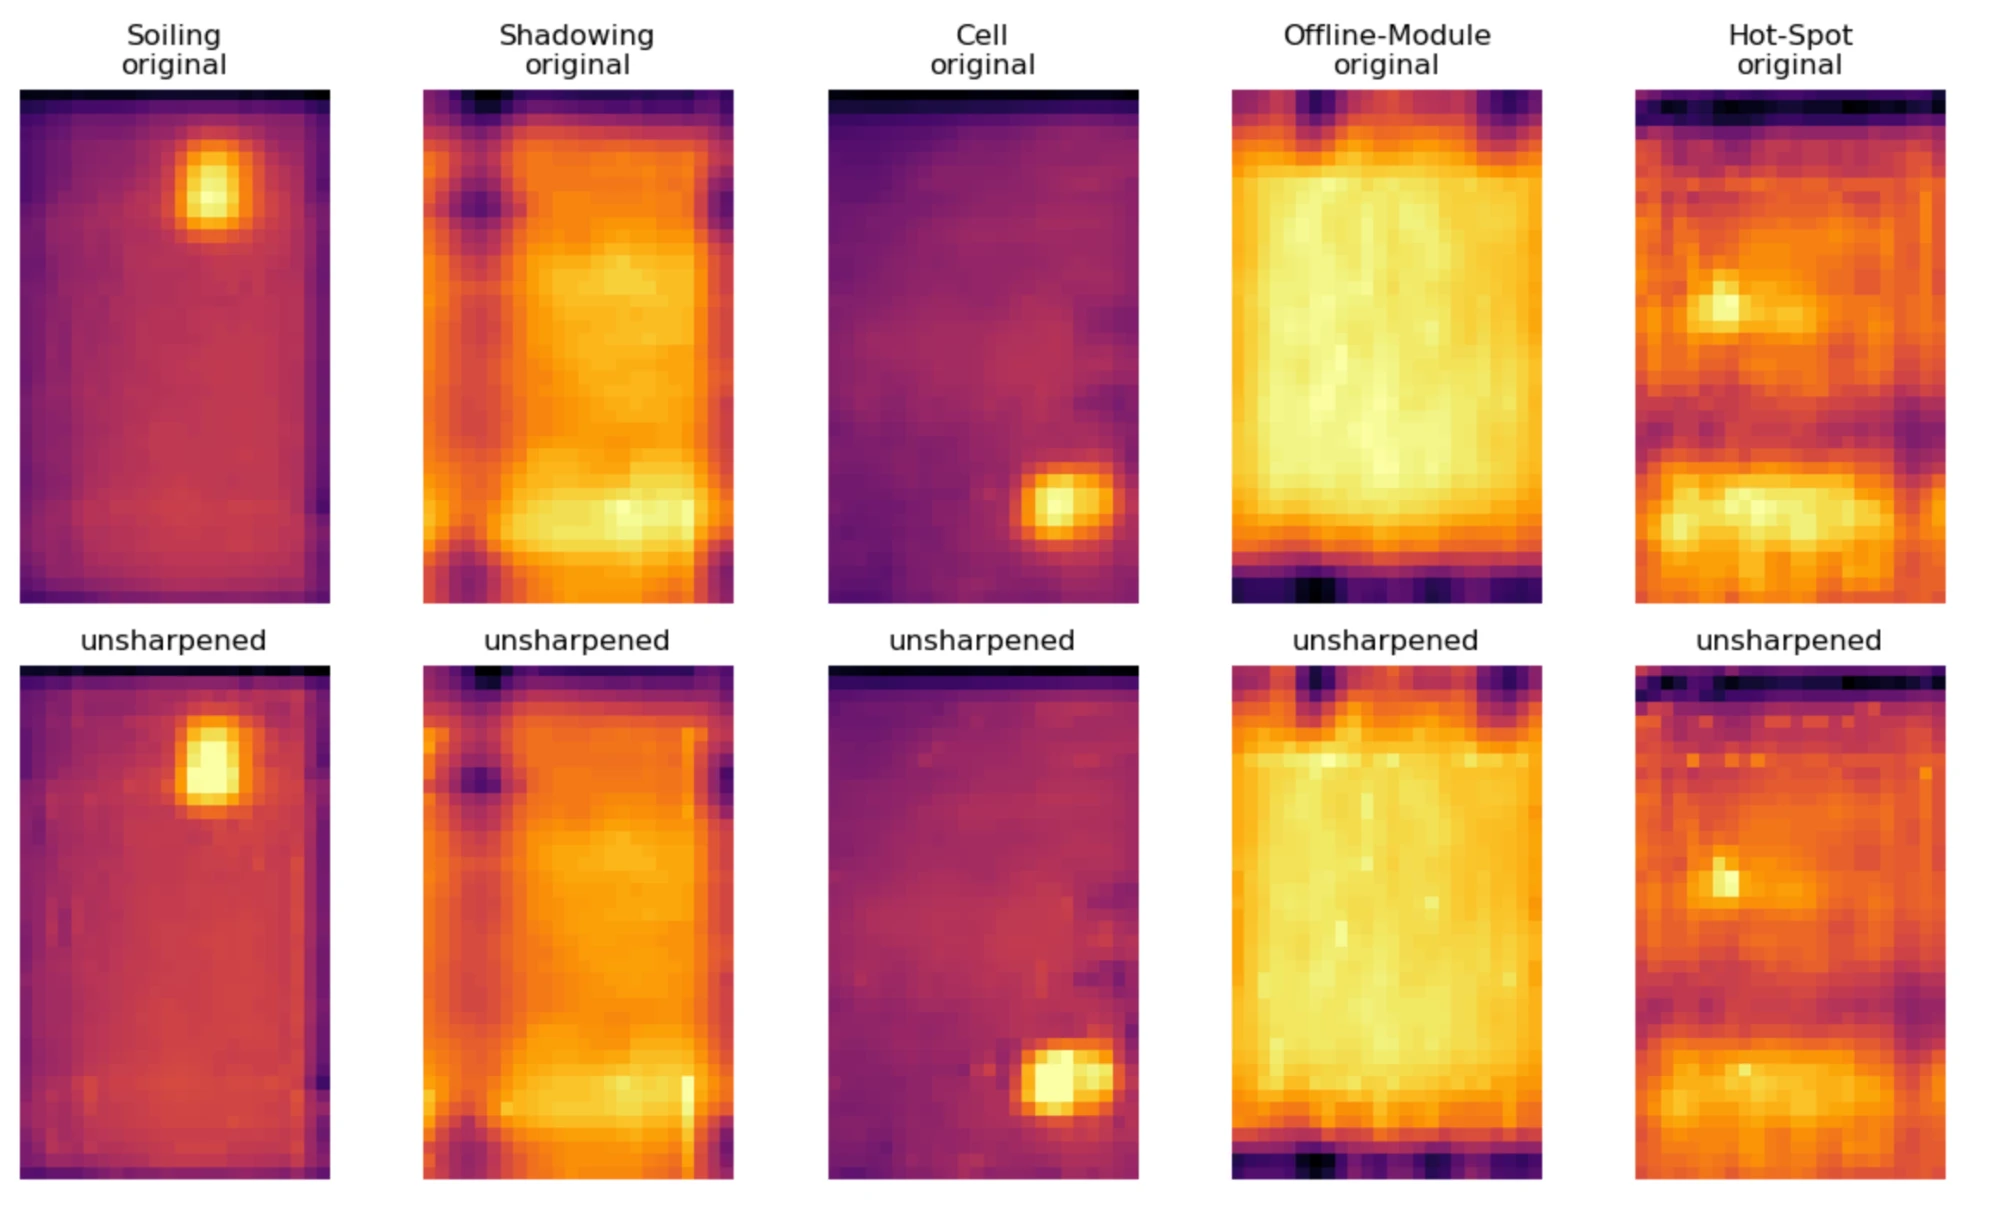
\includegraphics[width=\linewidth]{figs/p2_unsharp.png}
\caption{Unsharp masking (radius 1, amount 150\%, threshold 2). Top: original. Bottom: sharpened. The defects (hot spots, shadow edges) gain contrast and sharper boundaries.}
\label{fig:unsharp}
\end{figure}

\begin{figure}[t]
\centering
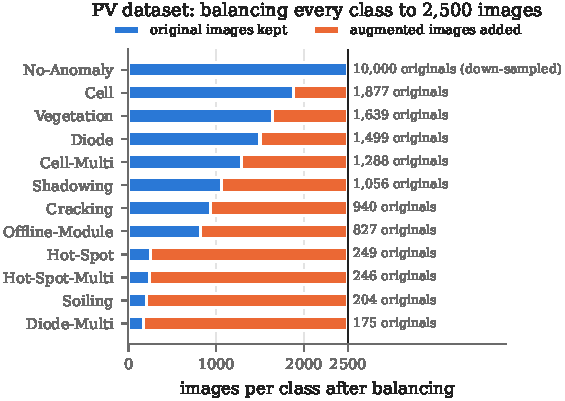
\includegraphics[width=\linewidth]{figs/p2_counts.pdf}
\caption{Class balancing to 2{,}500 images per class. Blue: original images kept. Orange: augmented images added.}
\label{fig:pv-counts}
\end{figure}

\begin{table}[t]
\centering\footnotesize\setlength{\tabcolsep}{4pt}
\begin{tabular}{@{}lrrrr@{}}
\toprule
Class & Before & Originals kept & Augmented & After \\
\midrule
No-Anomaly & 10{,}000 & 2{,}500 & 0 & 2{,}500 \\
Cell & 1{,}877 & 1{,}877 & 623 & 2{,}500 \\
Vegetation & 1{,}639 & 1{,}639 & 861 & 2{,}500 \\
Diode & 1{,}499 & 1{,}499 & 1{,}001 & 2{,}500 \\
Cell-Multi & 1{,}288 & 1{,}288 & 1{,}212 & 2{,}500 \\
Shadowing & 1{,}056 & 1{,}056 & 1{,}444 & 2{,}500 \\
Cracking & 940 & 940 & 1{,}560 & 2{,}500 \\
Offline-Module & 827 & 827 & 1{,}673 & 2{,}500 \\
Hot-Spot & 249 & 249 & 2{,}251 & 2{,}500 \\
Hot-Spot-Multi & 246 & 246 & 2{,}254 & 2{,}500 \\
Soiling & 204 & 204 & 2{,}296 & 2{,}500 \\
Diode-Multi & 175 & 175 & 2{,}325 & 2{,}500 \\
\midrule
Total & 20{,}000 & 12{,}500 & 17{,}500 & 30{,}000 \\
\bottomrule
\end{tabular}
\caption{Images per class before and after balancing and augmentation.}
\label{tab:pv}
\end{table}

\begin{lstlisting}[float=tbp,caption={Unsharp masking and augmentation (excerpt).},label={lst:aug}]
UNSHARP = ImageFilter.UnsharpMask(radius=1, percent=150,
                                  threshold=2)
AUGS = {"hflip": ImageOps.mirror, "vflip": ImageOps.flip,
        "jitter": T.ColorJitter(.2, .2)}  # bright., contr.
for c in classes:
    keep = originals[c]
    if len(keep) > 2500:                    # down-sample
        keep = rng.sample(keep, 2500)
    save([UNSHARP(load(p)) for p in keep])
    for _ in range(2500 - len(keep)):       # up-sample
        ops = rng.choice(non_empty_subsets(AUGS))
        src = UNSHARP(load(rng.choice(keep)))
        save(apply(ops, src))     # e.g. hflip+jitter
\end{lstlisting}

\subsection{ViT-B/32 fine-tuning strategies}
\label{sec:p2-2}
We fine-tune the ImageNet-1k pretrained ViT-B/32~\cite{dosovitskiy2021vit} (torchvision), replacing its head with a 12-way linear layer. The $24{\times}40$ images are replicated to 3 channels, resized to $224{\times}224$ (bilinear, on the GPU) and ImageNet-normalized, so each image becomes 49 patches of $32{\times}32$. All strategies use AdamW (weight decay 0.01), a one-cycle schedule with 10\% warm-up, batch 128, bfloat16 and 10 epochs, and we keep the epoch with the best validation accuracy. The learning rate is chosen per strategy, because a randomly initialized head needs a larger step than pretrained blocks:
\begin{enumerate}[nosep,leftmargin=*]
\item \textbf{Head only}: 9{,}228 trainable parameters (0.01\%), lr $10^{-3}$.
\item \textbf{Entire model}: 87.46M parameters (100\%), lr $5\cdot10^{-5}$.
\item \textbf{Last 4 blocks + final LayerNorm + head}: 28.36M parameters (32.4\%), lr $10^{-4}$.
\end{enumerate}

\begin{lstlisting}[float=tbp,caption={Selecting the trainable parameters for each strategy.},label={lst:freeze}]
m = vit_b_32(weights=ViT_B_32_Weights.IMAGENET1K_V1)
m.heads.head = nn.Linear(768, 12)
for p in m.parameters(): p.requires_grad = False
parts = {"head": [m.heads], "full": [m],
         "last": [m.heads, m.encoder.ln,
                  *m.encoder.layers[-4:]]}[strategy]
for part in parts:
    for p in part.parameters(): p.requires_grad = True
\end{lstlisting}

\begin{table}[t]
\centering\footnotesize\setlength{\tabcolsep}{3pt}
\begin{tabular}{@{}lrccccc@{}}
\toprule
Strategy & Trainable & Train & Val & Test & \makecell{Test\\(orig.)} & \makecell{Time\\(min)} \\
\midrule
1) Head only & 9.2K & 60.76 & 54.97 & 56.31 & 55.15 & \textbf{1.3} \\
2) Entire model & 87.5M & 99.94 & \textbf{71.83} & \textbf{73.25} & \textbf{76.37} & 4.2 \\
3) Last 4 blocks + head & 28.4M & 99.98 & 67.34 & 68.70 & 72.48 & 2.3 \\
\bottomrule
\end{tabular}
\caption{ViT-B/32 on the balanced PV dataset (accuracy in \%, 10 epochs, best validation epoch). ``Test (orig.)'' = the 1{,}875 non-augmented test images. Time = training time on one A100 MIG slice.}
\label{tab:vit-pv}
\end{table}

\begin{figure}[t]
\centering
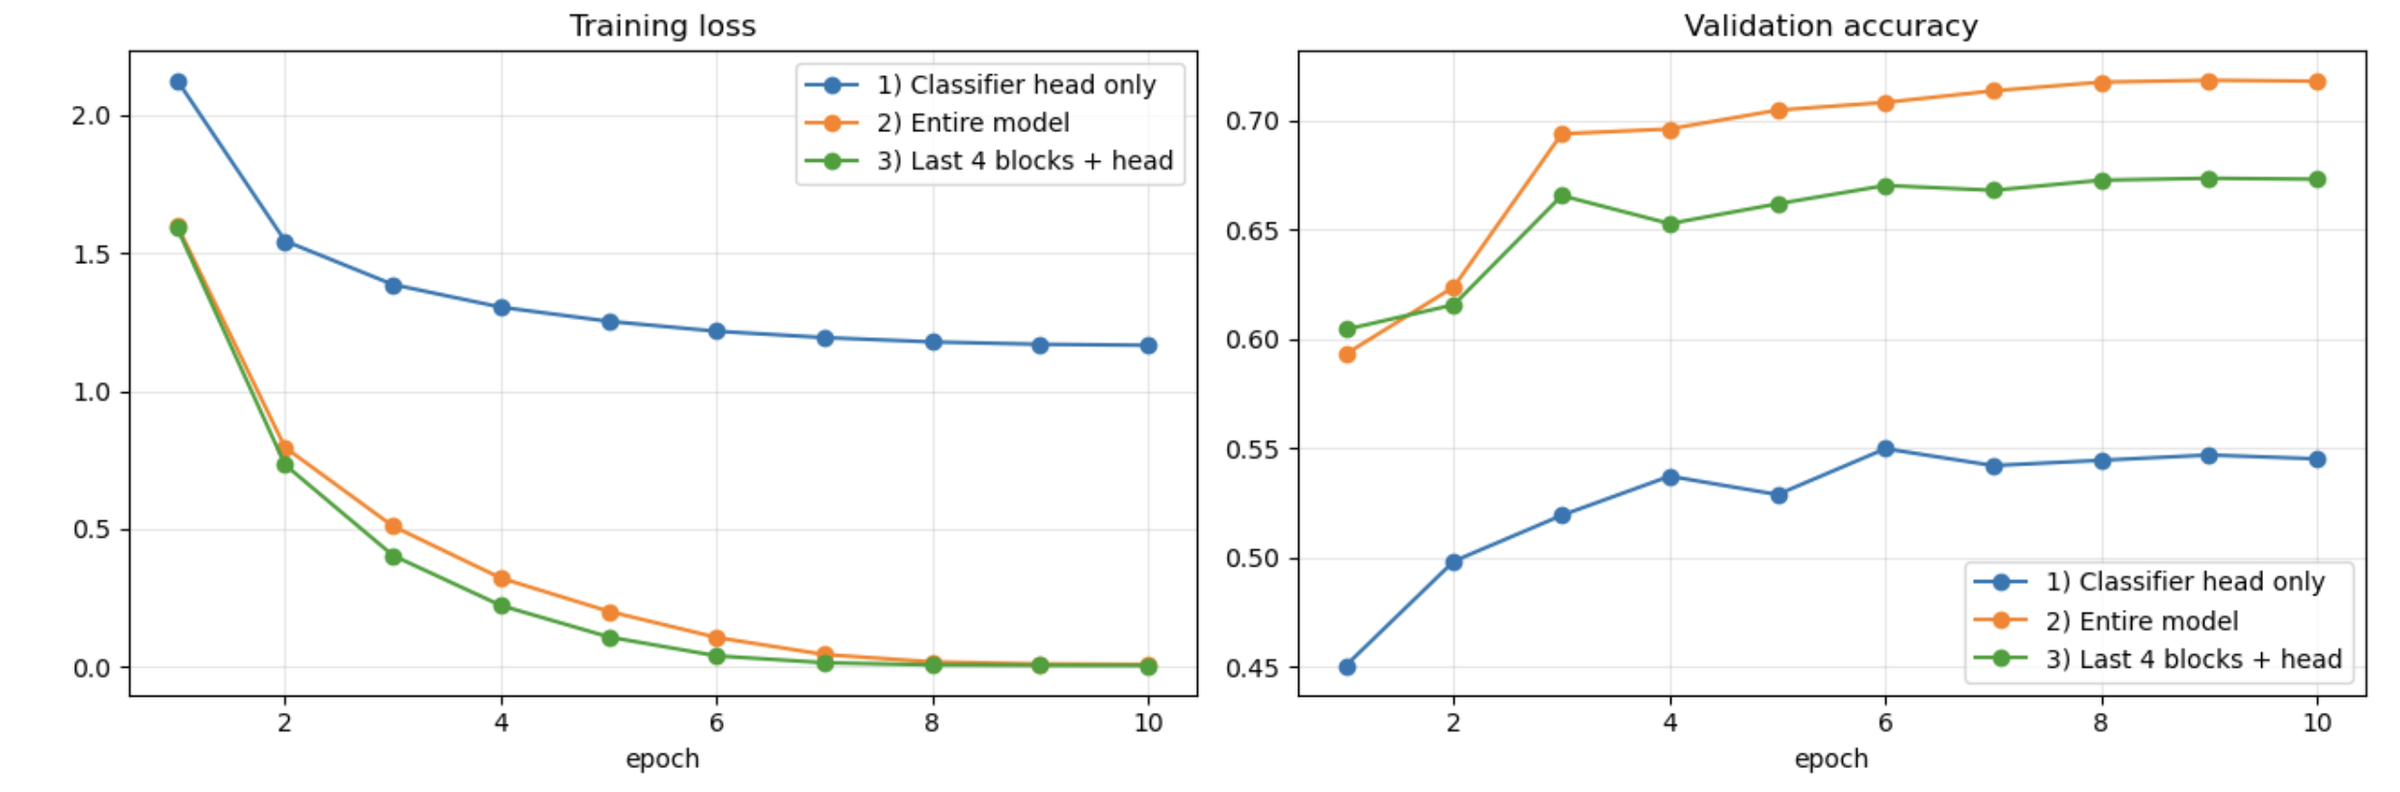
\includegraphics[width=\linewidth]{figs/p2_vit_curves.png}
\caption{ViT-B/32 learning curves. Left: training loss \vs epoch. Right: validation accuracy (fraction) \vs epoch. Head-only training plateaus at a high loss; the two strategies that adapt transformer blocks drive the training loss to $\approx$0 by epoch 8.}
\label{fig:vit-pv}
\end{figure}

\subsection{Analysis}
\label{sec:p2-3}
\paragraph{Accuracy.}
Fine-tuning the \textbf{entire model} gives the best accuracy (73.25\% test, 76.37\% on original images), 4.6 points above the \textbf{last 4 blocks} (68.70\%) and 16.9 points above the \textbf{head only} (56.31\%) (\cref{tab:vit-pv}, \cref{fig:vit-pv}). Validation and test agree within 1.5 points for every strategy, so the ranking is reliable.

\paragraph{Training efficiency.}
Training time grows with the depth of back-propagation: 1.3 min (head only), 2.3 min (last 4 of 12 blocks) and 4.2 min (all blocks). All three strategies run the same full forward pass, so the time grows less than the trainable-parameter count (9.2K, 28.4M and 87.5M). Optimizer memory, however, scales with the trainable parameters.

\paragraph{Why.}
(i)~\emph{Domain gap.} The images are upsampled $24{\times}40$ single-channel thermal maps, nothing like ImageNet photos. A linear head on frozen ImageNet features \emph{underfits}: training accuracy is only 60.8\% and the loss plateaus at $\approx$1.2, so the frozen representation does not separate the PV classes.
(ii)~\emph{Where to adapt.} Unfreezing the last 4 blocks lets the high-level features specialize, and the model fits the training set ($\approx$100\%). Full fine-tuning additionally adapts the patch embedding and early blocks to the blurry, low-contrast thermal patterns, which gives a further 4.5--4.6 points on validation and test. Since the first layers are where ImageNet and thermal images differ most, their adaptation matters.
(iii)~\emph{Overfitting.} Both unfrozen variants reach $\approx$100\% training accuracy while validation plateaus after epoch 3--6. They memorize the training set, especially the small classes, whose 2{,}500 images are mostly augmented copies of 175--250 originals. The best-validation checkpoint limits the damage.
(iv)~\emph{Hard classes.} The remaining errors are mostly counting problems (Cell \vs Cell-Multi, Hot-Spot \vs Hot-Spot-Multi) and Soiling (204 originals), as the ResNet-50 reference below shows.

\answer{Full fine-tuning is the most accurate (73.3\% test) and, at 4.2 min, still cheap on this small dataset. It is the best choice when accuracy matters. Fine-tuning the last 4 blocks is the best \emph{trade-off} when compute or memory is limited: 94\% of the full model's accuracy in 55\% of the time with 32\% of the trainable parameters. Training only the head is fastest but not usable (56.3\%), because frozen ImageNet features do not transfer to $24{\times}40$ thermal images.}

\paragraph{CNN reference (ResNet-50, full fine-tuning).}
To calibrate the ViT numbers we also fine-tuned all layers of an ImageNet ResNet-50 on the same split (\cref{tab:rn50}). The first version (AdamW, lr $10^{-4}$, $224{\times}224$ inputs) overfit after epoch 3: train accuracy reached 98\% while validation accuracy peaked at 63.9\%. Keeping the $24{\times}40$ aspect ratio ($224{\times}128$ inputs) and adding online flips and shifts, label smoothing 0.1, weight decay 0.05 and dropout 0.2 raised validation accuracy to 69.3\% and test accuracy from 67.2\% to 70.8\%. Test-time augmentation (averaging the original, h-flip and v-flip predictions) raised test accuracy to 72.6\%. The fully fine-tuned ViT-B/32 (73.3\%) is slightly better than the best ResNet-50, even without test-time augmentation. Per-class test accuracy of the improved model ranges from 96.3\% (Diode-Multi) and 92.1\% (Diode) down to 56.8\% (Hot-Spot-Multi), 50.4\% (Cell-Multi) and 44.7\% (Soiling). The largest confusions are Cell-Multi$\rightarrow$Cell (80), Soiling$\rightarrow$Cracking (78) and Hot-Spot-Multi$\rightarrow$Hot-Spot (67).

\begin{table}[t]
\centering\footnotesize\setlength{\tabcolsep}{3pt}
\begin{tabular}{@{}lcc@{}}
\toprule
ResNet-50 (all layers trained) & Test & Test (originals) \\
\midrule
baseline, $224{\times}224$, 10 epochs & 67.2 & 69.8 \\
improved, $224{\times}128$, 15 epochs & 70.8 & 73.6 \\
\quad + test-time augmentation & \textbf{72.6} & \textbf{75.7} \\
\midrule
ViT-B/32, entire model (\cref{tab:vit-pv}) & 73.3 & 76.4 \\
\bottomrule
\end{tabular}
\caption{CNN reference on the PV split (accuracy in \%). ``Originals'' = the 1{,}875 non-augmented test images.}
\label{tab:rn50}
\end{table}

%%%%%%%%%%%%%%%%%%%%%%%%%%%%%%%%%%%%%%%%%%%%%%%%%%%%%%%%%%%%%%%%%%%%%%%%%%%%%%%%%%%%%%%%%%%%%%%%%%%
\section{Problem 3: Custom ResNet on ImageNet}
\label{sec:p3}

\subsection{Prototype dataset}
\label{sec:p3-1}
\paragraph{Full split.}
The ImageNet training folder on Sol contains \textbf{650} class folders (not 1{,}000) with 832{,}571 images: at least 889 and at most 1{,}300 per class, with a median of 1{,}300. Class names come from the standard WordNet-ID$\rightarrow$name index. Because only this folder has labels, we split \emph{each class} 80/10/10 into train/val/test: 666{,}057 / 83{,}257 / 83{,}257 images. No image files are copied. The splits are CSV manifests (path, WordNet ID, label, split).

\paragraph{Prototype.}
We take \textbf{100 classes}, every 6.5-th WordNet ID in sorted order. Sorted IDs roughly group related concepts, so even spacing covers all super-categories instead of, for example, 100 dog breeds. We take \textbf{300 images per class} (240 train / 30 val / 30 test), sampled from the corresponding full splits, so every prototype test image is also a full-dataset test image. This gives 30{,}000 images (3.6\% of the data) with 24{,}000 / 3{,}000 / 3{,}000 in train/val/test. \cref{tab:proto} lists the statistics. A 30-epoch ResNet run on the prototype takes about 5 minutes on one A100, which makes design iteration fast. At the same time 240 images per class are enough to rank models, although the run-to-run spread is about $\pm$1 point (\cref{sec:p3-2}).

\begin{table}[t]
\centering\footnotesize\setlength{\tabcolsep}{4pt}
\resizebox{\linewidth}{!}{%
\begin{tabular}{@{}lr@{}}
\toprule
Classes (sampled every 6.5-th sorted WordNet ID) & 100 of 650 \\
Images per class (train / val / test) & 300 (240 / 30 / 30) \\
Total images (train / val / test) & 30{,}000 (24{,}000 / 3{,}000 / 3{,}000) \\
Fraction of the ImageNet folder on Sol & 3.6\% \\
Median image size (range) & $500{\times}375$ (W 62--3648, H 38--2851) \\
Color modes in a 3{,}000-image sample & RGB 98\%, grayscale 2\% \\
RGB mean (ImageNet reference) & 0.500, 0.467, 0.427 (0.485, 0.456, 0.406) \\
RGB std (ImageNet reference) & 0.281, 0.278, 0.295 (0.229, 0.224, 0.225) \\
\bottomrule
\end{tabular}}
\caption{Prototype dataset statistics.}
\label{tab:proto}
\end{table}

\begin{figure*}[t]
\centering
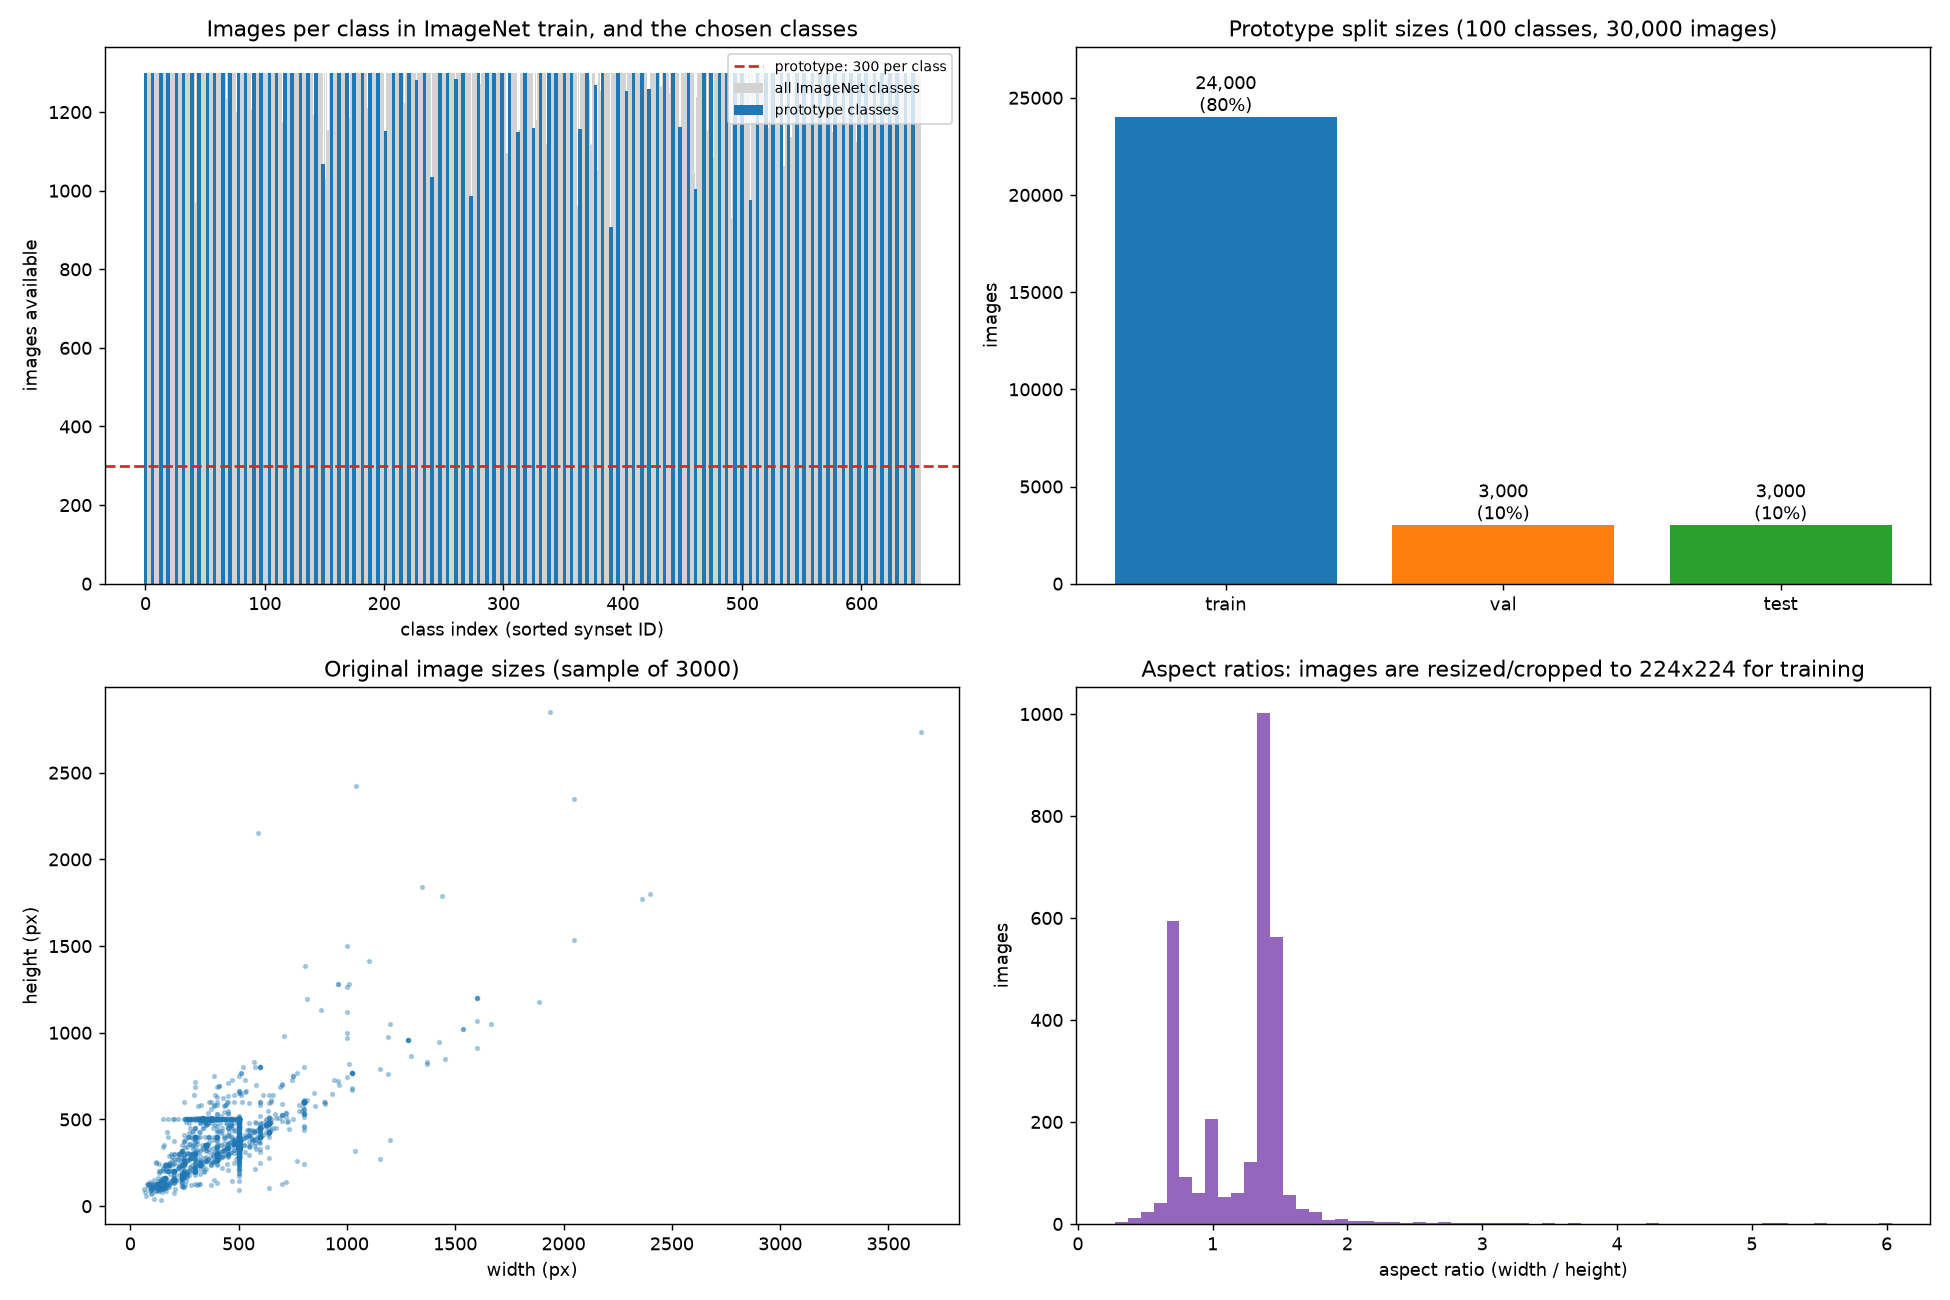
\includegraphics[width=0.49\linewidth]{figs/fig_proto_stats.png}\hfill
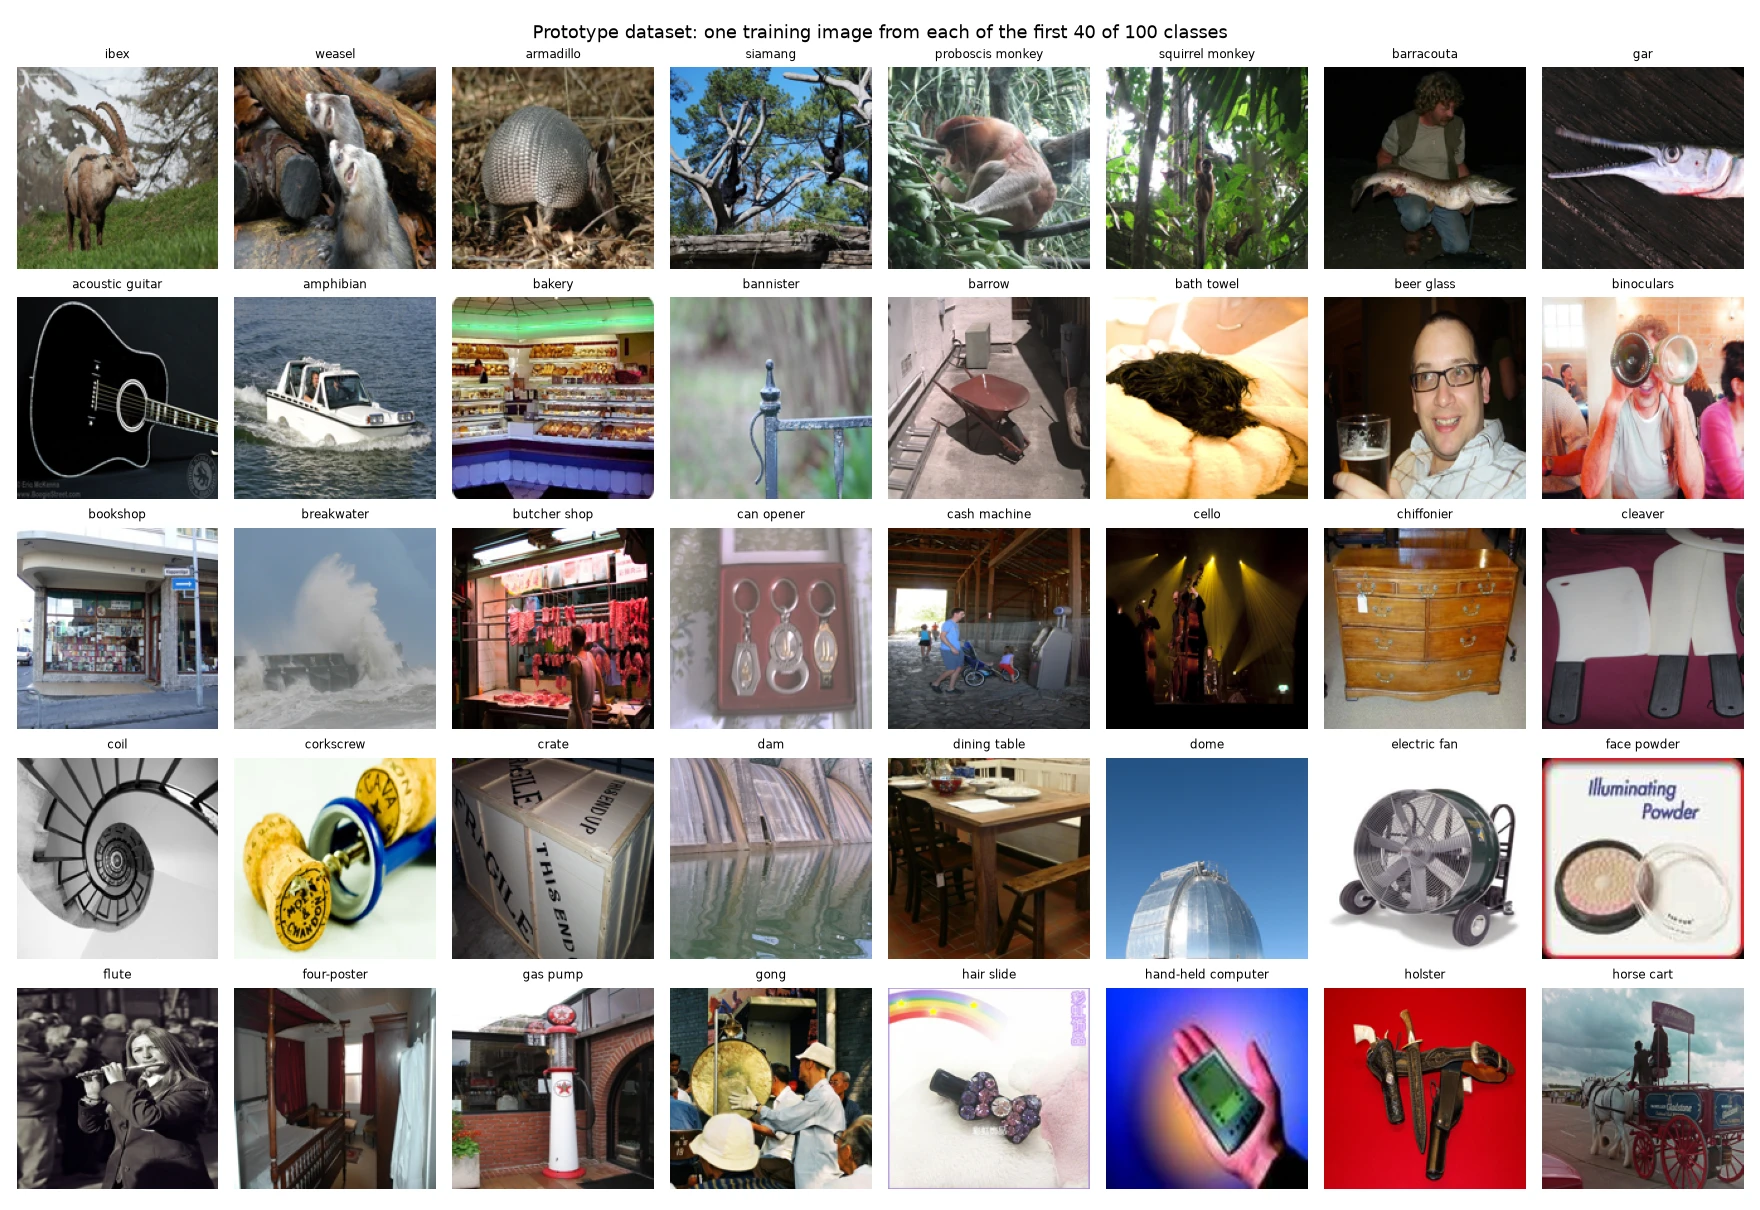
\includegraphics[width=0.49\linewidth]{figs/fig_proto_samples.png}
\caption{Prototype dataset. Left: images per class in Sol's ImageNet folder with the 100 selected classes (blue), split sizes, original image sizes and aspect ratios (sample of 3{,}000). Right: one training image from each of the first 40 prototype classes.}
\label{fig:proto}
\end{figure*}

\subsection{Custom ResNet-36}
\label{sec:p3-2}
\paragraph{Design.}
ResNet-34~\cite{he2016resnet} stacks $[3,4,6,3]$ BasicBlocks (two $3{\times}3$ convs each) in four stages: 1 stem conv + 32 block convs + 1 FC = 34 weighted layers. Our ResNet-36 uses $[3,4,\mathbf{7},3]$: one extra block in stage 3 (\cref{tab:arch}), giving 36 layers. 1$\times$1 shortcut convs are not counted, as in~\cite{he2016resnet}. The extra block adds 1.18M parameters (21.34M$\rightarrow$22.52M with a 100-class head) and about 0.23 GMACs, roughly 6\% of ResNet-34's compute. All weights are trained from scratch with Kaiming initialization, and the last BatchNorm of each block is zero-initialized so that every block starts as an identity map.

\paragraph{Expected benefit.}
Stage 3 works at $14{\times}14$ with 256 channels, where the network forms object-part representations. Deeper ResNets add depth mainly here (ResNet-101 has 23 stage-3 blocks), because it is the cheapest place to add capacity: each extra block costs the same compute as in other stages but has fewer parameters than a stage-4 block. We hoped the extra block would give a larger receptive field and one more non-linearity for composing parts. Residual connections should let the network ignore the block (identity map) if it does not help.

\begin{table}[t]
\centering\footnotesize\setlength{\tabcolsep}{4pt}
\resizebox{\linewidth}{!}{%
\begin{tabular}{@{}lcccc@{}}
\toprule
Stage & Output & Channels & ResNet-34 & \textbf{ResNet-36} \\
\midrule
stem: $7{\times}7$ conv /2, max-pool /2 & $56{\times}56$ & 64 & 1 conv & 1 conv \\
stage 1 & $56{\times}56$ & 64 & 3 blocks & 3 blocks \\
stage 2 & $28{\times}28$ & 128 & 4 blocks & 4 blocks \\
stage 3 & $14{\times}14$ & 256 & 6 blocks & \textbf{7 blocks} \\
stage 4 & $7{\times}7$ & 512 & 3 blocks & 3 blocks \\
head: avg-pool, FC & $1{\times}1$ & -- & 1 FC & 1 FC \\
\midrule
weighted layers / params (100 cl.) & & & 34 / 21.34M & 36 / 22.52M \\
\bottomrule
\end{tabular}}
\caption{ResNet-34 \vs our ResNet-36 for a $224{\times}224$ input. A block is two $3{\times}3$ conv layers with a skip connection.}
\label{tab:arch}
\end{table}

\paragraph{Training recipe (all prototype runs).}
SGD with Nesterov momentum 0.9, lr 0.05 (0.1 per 256 images, linearly scaled to batch 128~\cite{goyal2017imagenet1hour}), 2-epoch linear warm-up followed by cosine decay~\cite{loshchilov2017sgdr}, weight decay $5\cdot10^{-4}$ (not applied to BatchNorm parameters and biases), label smoothing 0.1~\cite{szegedy2016inception}, RandomResizedCrop $224$ + horizontal flip, batch 128 on one A100, and bfloat16. The model with the best validation top-1 is evaluated once on the test split.

\begin{table}[t]
\centering\footnotesize\setlength{\tabcolsep}{2.5pt}
\begin{tabular}{@{}lcccccc@{}}
\toprule
 & Ep. & Train & Val top-1/5 & Test top-1/5 & Gap & Time \\
\midrule
ResNet-34 & 30 & 57.4 & 52.7 / 77.5 & 53.5 / 79.0 & $-$3.9 & 5.1 \\
ResNet-36 & 30 & 57.6 & 53.5 / 77.6 & 53.4 / 78.7 & $-$4.2 & 5.1 \\
\midrule
ResNet-34 & 100 & 91.8 & 64.1 / 83.1 & 62.5 / 83.2 & 29.3 & 18.5 \\
 & & & {\tiny$\pm$0.0 / $\pm$0.1} & {\tiny$\pm$0.0 / $\pm$0.1} & & \\
ResNet-36 & 100 & 91.8 & 63.2 / 82.9 & \textbf{63.1} / 82.6 & 28.8 & 18.4 \\
 & & & {\tiny$\pm$0.0 / $\pm$0.2} & {\tiny$\pm$1.0 / $\pm$0.2} & & \\
\bottomrule
\end{tabular}
\caption{Depth comparison on the prototype (\%). 30-epoch runs: one seed. 100-epoch runs: mean $\pm$ s.e.\ over seeds 0 and 1. Gap = train $-$ test top-1. Time = training minutes on one A100.}
\label{tab:depth}
\end{table}

\paragraph{Results.}
\cref{tab:depth} and \cref{fig:proto-results} show that the two models are statistically indistinguishable. After 30 epochs they differ by 0.04 points in test top-1. After 100 epochs ResNet-36 is 0.6 points better on test top-1 but 0.9 points worse on validation. Both differences are smaller than the seed-to-seed variation: ResNet-36's test top-1 moved from 62.1\% to 64.0\% between seeds. The extra layers did not hurt optimization, since training accuracy is equal. Both models overfit heavily (about 92\% train \vs 62--63\% test), so on 240 images per class the bottleneck is data, not capacity, and one more block cannot be exploited.

\answer{ResNet-36 matches ResNet-34 on the prototype (test top-1 63.1\% \vs 62.5\%, within the $\pm$1-point seed noise) at +6\% compute. The benefit we hoped for, more part-level capacity in stage 3, cannot appear while both models are data-limited. We therefore keep ResNet-36 as the base model and test it at full scale (\cref{sec:p3-4}).}

\begin{figure}[t]
\centering
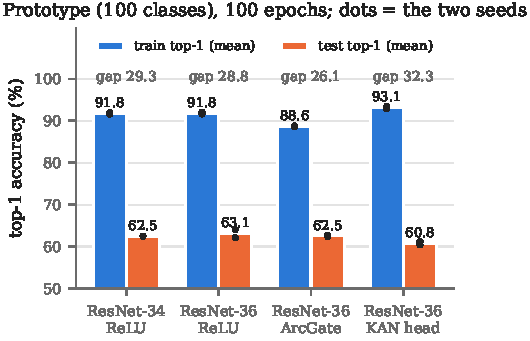
\includegraphics[width=\linewidth]{figs/p3_proto_results.pdf}
\caption{Train and test top-1 on the prototype after 100 epochs (bars: mean of 2 seeds; dots: individual seeds). ArcGate has the smallest train--test gap; the KAN head has the largest.}
\label{fig:proto-results}
\end{figure}

\subsection{Custom activation: ArcGate}
\label{sec:p3-3}
\paragraph{Definition.}
We propose
\begin{align}
\text{ArcGate}(x) &= x\,\Big(\frac12 + \frac1\pi\arctan x\Big), \\
f'(x) &= \frac12 + \frac{\arctan x}{\pi} + \frac{x}{\pi(1+x^2)} .
\end{align}
The gate $\tfrac12+\tfrac1\pi\arctan x$ is the CDF of the standard \emph{Cauchy} distribution. ArcGate is thus the heavy-tailed member of the self-gating family $x\,\Phi(x)$ that includes GELU (Gaussian CDF)~\cite{hendrycks2016gelu} and SiLU/Swish (logistic CDF)~\cite{ramachandran2017swish}. It is not available in PyTorch. Its properties (\cref{fig:arcgate}):
\begin{itemize}[nosep,leftmargin=*]
\item $f(0)=0$, $f'(0)=\tfrac12$, and $f(x)\approx x-\tfrac1\pi$ for large positive $x$, so it behaves like ReLU for strong activations.
\item It is monotonic and bounded below by $-1/\pi\approx-0.318$, approached as $x\to-\infty$ (expansion: $f(x)=-\tfrac1\pi+\tfrac{1}{3\pi x^2}+\dots$). Unlike SiLU and GELU, it has no negative dip.
\item For negative inputs the gradient decays only polynomially, $f'(x)\approx\tfrac{2}{3\pi|x|^3}$, instead of exponentially (SiLU/GELU) or to exactly 0 (ReLU). Units therefore never ``die'', and negative pre-activations still receive a learning signal.
\end{itemize}

\paragraph{Expectations.}
Compared with ReLU we expected (i) smoother optimization, because the gradient is continuous at 0; (ii) no dead units; and (iii) a mild regularization effect, because the soft gate passes small negative values and the network cannot easily form the sharp, sparse codes that support memorization. We expected similar or slightly better accuracy, at a small compute cost for $\arctan$.

\begin{figure*}[t]
\centering
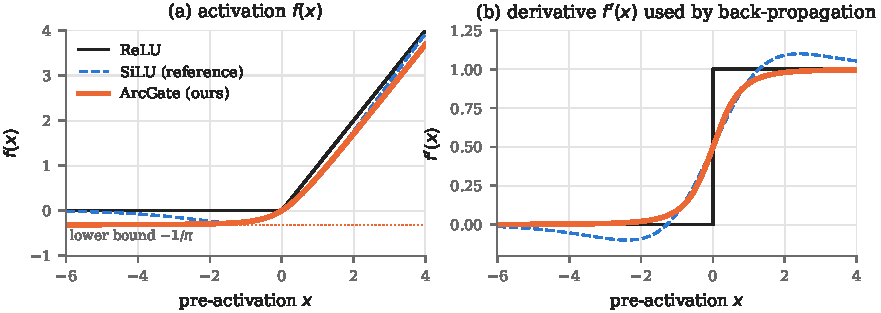
\includegraphics[width=\linewidth]{figs/p3_activation.pdf}
\caption{ArcGate compared with ReLU (and SiLU for reference). (a) ArcGate is smooth, monotonic, passes small negative values and is bounded below by $-1/\pi$. (b) Its derivative rises smoothly from 0 to 1 and, unlike ReLU's, is never exactly zero.}
\label{fig:arcgate}
\end{figure*}

\paragraph{Implementation.}
ArcGate replaces every ReLU in ResNet-36. We use a custom \texttt{autograd.Function} that stores only the input $x$ and recomputes $f'(x)$ in the backward pass (\cref{lst:arcgate}). This keeps activation memory equal to ReLU's.

\begin{lstlisting}[float=tbp,caption={ArcGate with a hand-written backward pass.},label={lst:arcgate}]
class _ArcGateFn(torch.autograd.Function):
    @staticmethod
    def forward(ctx, x):
        ctx.save_for_backward(x)
        return x * (0.5 + torch.atan(x) / math.pi)
    @staticmethod
    def backward(ctx, g):
        (x,) = ctx.saved_tensors
        return g * (0.5 + torch.atan(x) / math.pi
                    + x / (math.pi * (1 + x * x)))
\end{lstlisting}

\begin{table}[t]
\centering\footnotesize\setlength{\tabcolsep}{2.5pt}
\begin{tabular}{@{}lccccc@{}}
\toprule
ResNet-36, 100 ep. & Train & Val top-1/5 & Test top-1/5 & Gap & Time \\
\midrule
ReLU & 91.8 & 63.2 / 82.9 & 63.1 / 82.6 & 28.8 & 18.4 \\
 & & {\tiny$\pm$0.0 / $\pm$0.2} & {\tiny$\pm$1.0 / $\pm$0.2} & & \\
\textbf{ArcGate} & 88.6 & 63.2 / \textbf{83.5} & 62.5 / \textbf{83.6} & \textbf{26.1} & 20.3 \\
 & & {\tiny$\pm$0.5 / $\pm$0.2} & {\tiny$\pm$0.1 / $\pm$0.0} & & \\
ReLU + KAN head & 93.1 & 60.7 / 80.1 & 60.8 / 80.8 & 32.3 & 17.9 \\
 & & {\tiny$\pm$0.4 / $\pm$0.2} & {\tiny$\pm$0.4 / $\pm$0.1} & & \\
\bottomrule
\end{tabular}
\caption{Activation comparison on the prototype (\%, mean $\pm$ s.e.\ over 2 seeds). Gap = train $-$ test top-1. Time = minutes per 100-epoch run (seed 0).}
\label{tab:act}
\end{table}

\paragraph{Results.}
\cref{tab:act} shows that ArcGate matches ReLU in top-1: validation accuracy is identical (63.2\%), and the test difference ($-$0.5) is within ReLU's own $\pm$1.0 seed variation. ArcGate improves top-5 accuracy in both seeds and on both evaluation sets (+0.6 validation, +1.1 test). Its most robust effect is \emph{less overfitting}. It reaches the same test accuracy with about 3 points lower training accuracy (88.6\% \vs 91.8\%), which shrinks the train--test gap from 28.8 to 26.1 points; the reduction appears in both seeds (25.9 and 26.3 \vs 29.5 and 28.0). This is the regularizing effect we expected from a soft gate that never blocks the gradient completely. The cost is 10\% longer training (20.3 \vs 18.4 min), from the $\arctan$ computation.

\paragraph{Extra: KAN classifier head.}
We also replaced the final FC layer with a Kolmogorov--Arnold layer~\cite{liu2024kan}. Each input--output pair gets a learnable function $w\,\text{SiLU}(x)+\sum_k c_k B_k(x)$, where $B_k$ are cubic B-splines on a 5-interval grid over $[-3,3]$, preceded by a LayerNorm. The head adds 0.41M parameters. It was consistently worse ($-$2.3 test top-1, $-$1.8 top-5) and overfit the most (gap 32.3), because a more flexible head memorizes the 240 images per class more easily.

\answer{ArcGate is a new Cauchy-gated activation. It matches ReLU in top-1 accuracy, gives a small but consistent top-5 gain (+1.1 test points), and reduces overfitting by 2.7 points in both seeds, at 10\% extra training time. We use ResNet-36 + ArcGate for the full-dataset runs.}

\subsection{Full ImageNet on GPUs and Gaudi accelerators}
\label{sec:p3-4}
\paragraph{Setup.}
ResNet-36 + ArcGate (22.80M parameters, 650-way head) is trained from scratch on the full split (666{,}057 training images) for 10 epochs with distributed data-parallel training on two devices, in two separate runs:
(i)~2$\times$NVIDIA A100-SXM4-80GB with NCCL, and
(ii)~2$\times$Intel Gaudi~2 (HL-225) with HCCL in \emph{lazy mode}~\cite{habana2025docs}. Lazy mode collects operations into a graph and executes it at each \texttt{htcore.mark\_step()} (\cref{lst:gaudi}).
Both runs use identical hyperparameters (\cref{tab:hparams}) and the same split and seed, so the platforms are directly comparable. JPEG decoding uses 14 loader processes per device. The model is selected on the validation split and evaluated \emph{once} on the 83{,}257-image test split.

\begin{table}[t]
\centering\footnotesize\setlength{\tabcolsep}{4pt}
\begin{tabular}{@{}ll@{}}
\toprule
Model & ResNet-36 [3,4,7,3], ArcGate, 22.80M params \\
Data & 650 classes; 666{,}057 / 83{,}257 / 83{,}257 images \\
Epochs & 10 \\
Batch & 128 per device $\times$ 2 devices = 256 \\
Optimizer & SGD, Nesterov momentum 0.9 \\
Learning rate & 0.1, 1-epoch linear warm-up, cosine decay to 0 \\
Weight decay & $10^{-4}$ (none on BatchNorm and biases) \\
Regularization & label smoothing 0.1 \\
Augmentation & RandomResizedCrop 224, horizontal flip \\
Evaluation & resize 256, center crop 224 \\
Precision & bfloat16 autocast \\
\bottomrule
\end{tabular}
\caption{Hyperparameters of the full-ImageNet runs (identical on A100 and Gaudi~2).}
\label{tab:hparams}
\end{table}

\begin{lstlisting}[float=tbp,caption={Gaudi-specific parts of the training loop and job script (excerpt).},label={lst:gaudi}]
import habana_frameworks.torch.core as htcore
dist.init_process_group("hccl")
model = DDP(model.to("hpu"), bucket_cap_mb=100,
            gradient_as_bucket_view=True)
loss.backward();  htcore.mark_step()   # run the graph
opt.step();       htcore.mark_step()
# SBATCH: -p gaudi -q class_gaudi --gres=gpu:hl225:2
# export PT_HPU_LAZY_MODE=1
# torchrun --nproc_per_node 2 train_imagenet.py ...
\end{lstlisting}

\begin{table}[t]
\centering\footnotesize\setlength{\tabcolsep}{4pt}
\resizebox{\linewidth}{!}{%
\begin{tabular}{@{}lcc@{}}
\toprule
 & 2$\times$A100 & 2$\times$Gaudi~2 \\
\midrule
Train top-1 (augmented images) & 54.43 & 54.33 \\
Val top-1 / top-5 & 59.97 / 82.56 & 59.75 / 82.32 \\
\textbf{Test top-1 / top-5} & \textbf{60.38 / 82.87} & \textbf{60.28 / 82.76} \\
Best epoch & 10 / 10 & 10 / 10 \\
\midrule
Training time, 10 epochs & 53.9 min & \textbf{46.8 min} \\
Whole job (incl.\ test + latency) & 63.1 min & \textbf{52.6 min} \\
Training throughput & 2{,}121 img/s & \textbf{2{,}381 img/s} \\
\midrule
Latency, batch 1 (mean / p50 / p90) & \textbf{6.21} / 6.19 / 6.28 ms & 9.15 / 9.15 / 9.19 ms \\
Latency, batch 64 (mean / p50 / p90) & \textbf{7.72} / 7.65 / 8.18 ms & 9.35 / 9.12 / 9.18 ms \\
Inference throughput, batch 64 & \textbf{8{,}286 img/s} & 6{,}844 img/s \\
\bottomrule
\end{tabular}}
\caption{Full-ImageNet results for ResNet-36 + ArcGate (accuracy in \%). Latency is measured on one device with bfloat16 and a $224{\times}224$ input, after 20 warm-up iterations, over 100 timed forward passes, excluding data loading.}
\label{tab:full}
\end{table}

\begin{figure}[t]
\centering
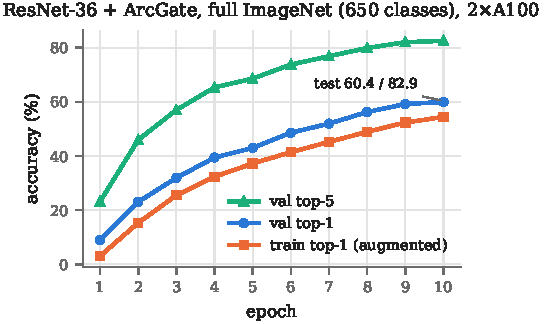
\includegraphics[width=\linewidth]{figs/p3_full_curve.pdf}
\caption{Full-ImageNet training curve (A100 run). Validation accuracy is still rising at epoch 10, and train accuracy (measured on augmented crops with label smoothing) stays below validation accuracy, so the model is not overfitting.}
\label{fig:full-curve}
\end{figure}

\begin{figure*}[t]
\centering
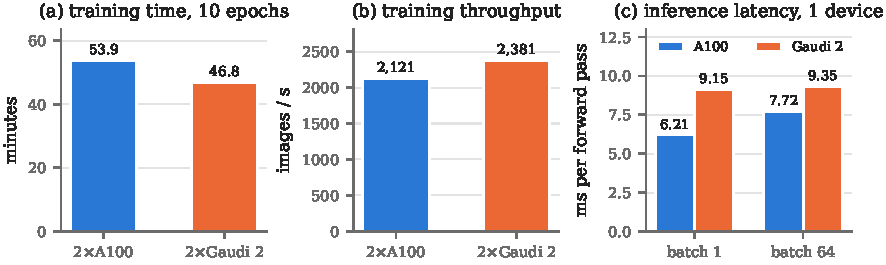
\includegraphics[width=\linewidth]{figs/p3_gpu_gaudi.pdf}
\caption{A100 \vs Gaudi~2 with identical model, data and hyperparameters. Gaudi~2 trains 13\% faster, while the A100 has lower single-device inference latency at both batch sizes.}
\label{fig:gpu-gaudi}
\end{figure*}

\paragraph{Results.}
\cref{tab:full} and \cref{fig:full-curve,fig:gpu-gaudi} summarize the results.
\emph{Accuracy.} Both platforms reach the same accuracy: test top-1 differs by 0.10 points and top-5 by 0.11 points, which is within run-to-run noise (data order, bfloat16 rounding). The model therefore transfers to Gaudi without loss. With 28$\times$ more training images (and 6.5$\times$ more classes) than the prototype, it reaches 60.4\% top-1 in only 10 epochs. The best epoch is the last one, so longer training would improve accuracy further.
\emph{Training speed.} Gaudi~2 finished the 10 epochs 13\% faster (46.8 \vs 53.9 min, 2{,}381 \vs 2{,}121 img/s). Training at this scale is partly limited by CPU JPEG decoding, so part of the gap may come from the Gaudi node's CPUs and storage rather than from the accelerator itself.
\emph{Latency.} The A100 is faster at inference: 6.2 \vs 9.2 ms at batch 1 and 8{,}286 \vs 6{,}844 img/s at batch 64. On Gaudi the batch-1 and batch-64 latencies are almost equal (9.15 \vs 9.12 ms median). This indicates a fixed per-call cost of about 9 ms for graph launch in lazy mode, which dominates small batches. Gaudi throughput scales 63$\times$ from batch 1 to batch 64 at nearly constant latency.

\answer{ResNet-36 + ArcGate was trained for 10 epochs on full ImageNet (650 classes). It reaches 60.4\% / 82.9\% test top-1 / top-5 on A100 and 60.3\% / 82.8\% on Gaudi~2. Training took 53.9 min on 2$\times$A100 and 46.8 min on 2$\times$Gaudi~2. Batch-1 latency is 6.2 ms (A100) and 9.2 ms (Gaudi~2).}

\subsection{Vision transformer \vs custom ResNet}
\label{sec:p3-5}
\paragraph{Model and recipe.}
We implement ViT-S/16~\cite{dosovitskiy2021vit,touvron2021deit}: $16{\times}16$ patches (196 tokens + class token), 12 transformer blocks, 6 heads, width 384, MLP width 1{,}536, and 21.9M parameters. This size was chosen to match ResNet-36 (22.8M). It is trained from scratch with the standard ViT recipe: AdamW (lr $1.25\cdot10^{-4}$ for batch 128, i.e.\ $5\cdot10^{-4}$ per 512 images, linearly scaled), weight decay 0.05, gradient clipping 1.0, warm-up (5 epochs on the prototype, 1 on the full set) followed by cosine decay, and label smoothing 0.1. Data, augmentation, epochs and seed are identical to the ResNet runs. It ran on one A100 with batch 128.

\begin{table}[t]
\centering\footnotesize\setlength{\tabcolsep}{2.6pt}
\begin{tabular}{@{}llcc@{}}
\toprule
 & & \makecell{ResNet-36\\+ArcGate} & \makecell{ViT-S/16\\(ours)} \\
\midrule
\multicolumn{2}{@{}l}{Parameters (100 / 650 classes)} & 22.5 / 22.8M & 21.7 / 21.9M \\
\multicolumn{2}{@{}l}{Depth} & 36 layers & 12 blocks \\
\midrule
\multirow{4}{*}{\makecell[l]{Prototype\\100 ep.}} & Train top-1 & 88.6 & 87.5 \\
 & Val top-1 / top-5 & 62.8 / 83.3 & 36.4 / 58.0 \\
 & \textbf{Test top-1 / top-5} & \textbf{62.7 / 83.7} & 35.6 / 59.6 \\
 & Train time (1 A100) & 20.3 min & 23.1 min \\
\midrule
\multirow{6}{*}{\makecell[l]{Full\\ImageNet\\10 ep.}} & Train top-1 & 54.4 & 44.5 \\
 & Val top-1 / top-5 & 60.0 / 82.6 & 45.2 / 69.7 \\
 & \textbf{Test top-1 / top-5} & \textbf{60.4 / 82.9} & 45.4 / 70.0 \\
 & Train time (devices) & 53.9 min (2) & 59.1 min (1) \\
 & Latency, batch 1 & 6.21 ms & \textbf{5.74 ms} \\
 & Latency, batch 64 & \textbf{7.72 ms} & 10.53 ms \\
\bottomrule
\end{tabular}
\caption{Custom ResNet \vs ViT trained from scratch (seed 0, accuracy in \%, latency on one A100 in bfloat16).}
\label{tab:vit}
\end{table}

\begin{figure}[t]
\centering
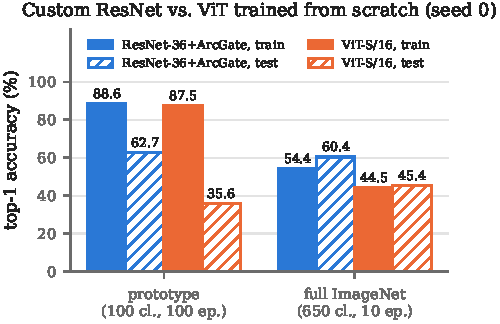
\includegraphics[width=\linewidth]{figs/p3_vit_vs_resnet.pdf}
\caption{Train (solid) and test (hatched) top-1 for ResNet-36+ArcGate and ViT-S/16. On the prototype the ViT fits the training set as well as the ResNet but generalizes poorly. With 28$\times$ more data the gap shrinks and the ViT no longer overfits.}
\label{fig:vit}
\end{figure}

\paragraph{Results.}
The ViT does \emph{not} outperform our ResNet (\cref{tab:vit}, \cref{fig:vit}). On the prototype both models fit the training set equally well (88.6\% \vs 87.5\%), but the ViT reaches only 35.6\% test top-1 against 62.7\%. Its generalization gap is 52 points and its best validation epoch is 62 of 100. With 650 classes and 666k images the gap shrinks from 27 to 15 points (60.4\% \vs 45.4\%), and the ViT no longer overfits (train 44.5\% $<$ test 45.4\%). Its best epoch is also the last, so it is underfitting. The explanation is inductive bias: convolutions build in locality and translation equivariance, while a ViT must learn from data that neighboring patches are related. This requires far more data or longer training: the original ViT pre-trained on 14--300M images, and DeiT used 300 epochs with strong augmentation~\cite{dosovitskiy2021vit,touvron2021deit}.
For a single image the ViT is 8\% faster (5.74 \vs 6.21 ms). It runs 12 wide blocks, while the ResNet runs 36 sequential layers, which adds launch overhead. At batch 64 the ResNet is 36\% faster, because attention and MLPs over 197 tokens cost more compute than the ResNet's convolutions. Note that the full-data ViT trained on one GPU (batch 128) and the ResNet on two (batch 256), so their training times are not directly comparable.

\answer{No. At matched size ($\sim$22M parameters) and an identical 10-epoch budget, ResNet-36 + ArcGate beats ViT-S/16 by 15.0 points in top-1 (60.4\% \vs 45.4\%) and 12.9 points in top-5, and has 36\% higher batch-64 throughput. The ViT is slightly faster at batch 1, and its deficit shrinks as data grows (27 $\rightarrow$ 15 points).}

%%%%%%%%%%%%%%%%%%%%%%%%%%%%%%%%%%%%%%%%%%%%%%%%%%%%%%%%%%%%%%%%%%%%%%%%%%%%%%%%%%%%%%%%%%%%%%%%%%%
\section{Conclusion}
Pixel losses and raw VGG features disagree about what a ``small'' change is. Much of VGG's sensitivity to imperceptible shifts comes from aliasing, which motivated the anti-aliased, contrastively trained turbulence feature. On PV infrared data, class balancing with grouped (leakage-free) splits is essential, and fine-tuning strategies trade accuracy against compute. On ImageNet, a soft Cauchy-gated activation regularizes as well as it fits. The same model trains to identical accuracy on A100 and Gaudi~2, faster on Gaudi. Convolutional inductive bias remains decisive against a ViT trained from scratch at this data and compute budget.

%%%%%%%%%%%%%%%%%%%%%%%%%%%%%%%%%%%%%%%%%%%%%%%%%%%%%%%%%%%%%%%%%%%%%%%%%%%%%%%%%%%%%%%%%%%%%%%%%%%
\section*{Acknowledgements}
\noindent\textbf{Data and code.} RaptorMaps InfraredSolarModules dataset~\cite{millendorf2020pv}; DIV2K~\cite{agustsson2017div2k}; DAATSim simulator (\url{https://github.com/Riponcs/DAATSim})~\cite{saha2025daatsim}; ImageNet~\cite{deng2009imagenet} as provided on Sol; PyTorch and torchvision~\cite{paszke2019pytorch} (pretrained VGG-16, ViT-B/32, ResNet-50); the KAN layer follows~\cite{liu2024kan}.
\textbf{Documentation.} ASU Research Computing Sol and SBATCH documentation~\cite{asurc2025sol}; the course's Gaudi example script (Lab~14); Intel Gaudi documentation~\cite{habana2025docs}; the CVPR 2026 author kit for this template.
\textbf{Compute.} ASU Research Computing (Sol A100 GPUs and Gaudi~2 nodes); the instructor granted the \texttt{class\_gaudi} QOS.
\textbf{AI assistance.} Claude (Anthropic), an AI assistant, was used to help write and debug code and Slurm job scripts and to draft this report. All experiments were run, and all numbers produced, by the author on Sol.
\textbf{Classmates.} \TODO{list any classmate help, or write ``None''.}

{
    \small
    \bibliographystyle{ieeenat_fullname}
    \bibliography{main}
}

\end{document}
